% Phụ lục D (phần sơ đồ) — ERD theo từng miền, chuyển từ thân Chương 5; hình sinh từ tools/diagrams/gen_erd.py.

\subsection*{Sơ đồ ERD theo miền}

Mỗi bảng chỉ hiện khóa chính, khóa ngoại, tối đa một hai cột định danh (mã, trạng thái) và một dòng mô tả; các cột còn lại ghi ``+N cột khác'' và có đủ trong từ điển trên. Nét liền là khóa ngoại thật giữa hai bảng cùng schema; nét đứt là tham chiếu sang schema khác bằng định danh, không có khóa ngoại vật lý (ràng buộc RB3, mục~\ref{sec:kientruc}); đường nét đứt chỉ vẽ khi đích nằm cùng hình và không vẽ tới bảng được từ bốn bảng trở lên trỏ vào (như \texttt{identity.users}). Hai đầu mỗi đường theo ký hiệu chân chim: phía bảng cha, hai gạch là đúng một (khóa ngoại \texttt{NOT NULL}), gạch kèm vòng tròn là không hoặc một (cho phép \texttt{NULL}); phía bảng con, chân chim kèm vòng tròn là không hoặc nhiều. Vòng nhỏ sát mép bảng là khóa ngoại trỏ về chính bảng đó. Bảng chỉ thiết kế vẽ nét đứt nền xám.

\begin{figure}[t]
\centering
\begin{adjustbox}{max totalsize={\textwidth}{0.47\textheight},center}
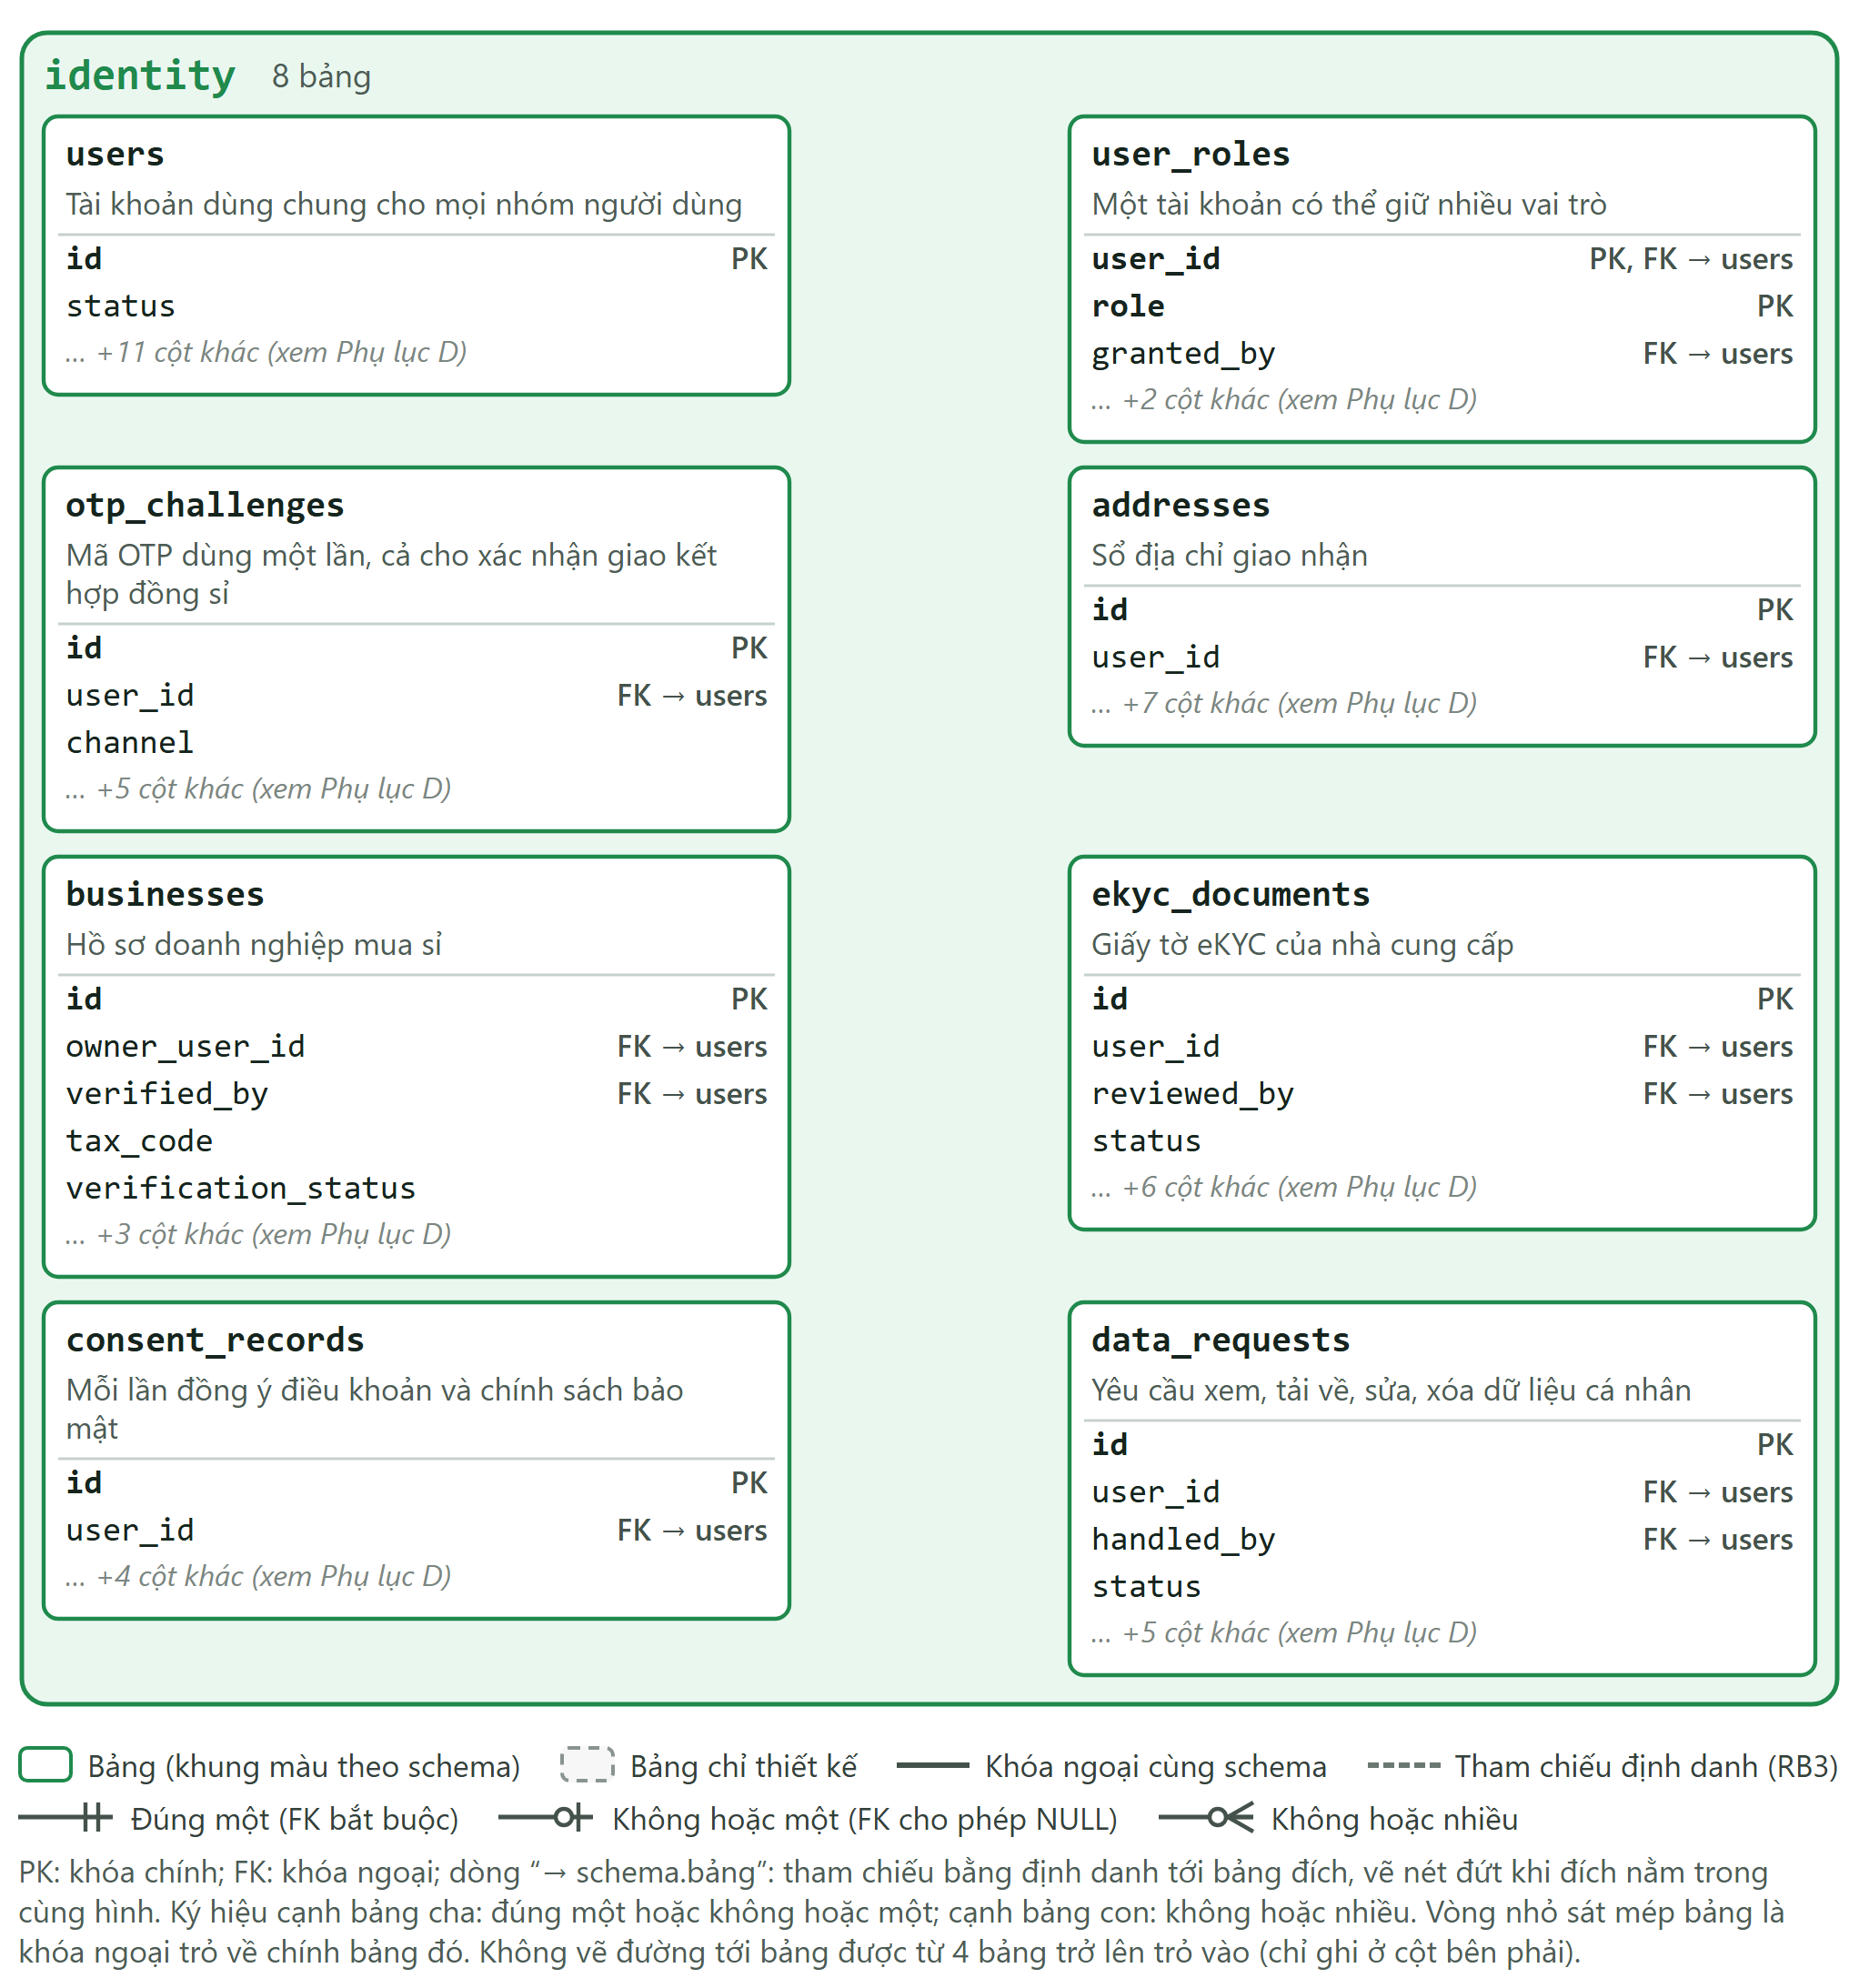
\includegraphics[width=\textwidth]{image/comparison/erd-dinh-danh.png}
\end{adjustbox}
\caption{ERD nền tảng chung, schema \texttt{identity} (8 bảng)}
\label{fig:erd-dinh-danh}
\end{figure}

\begin{figure}[t]
\centering
\begin{adjustbox}{max totalsize={\textwidth}{0.47\textheight},center}
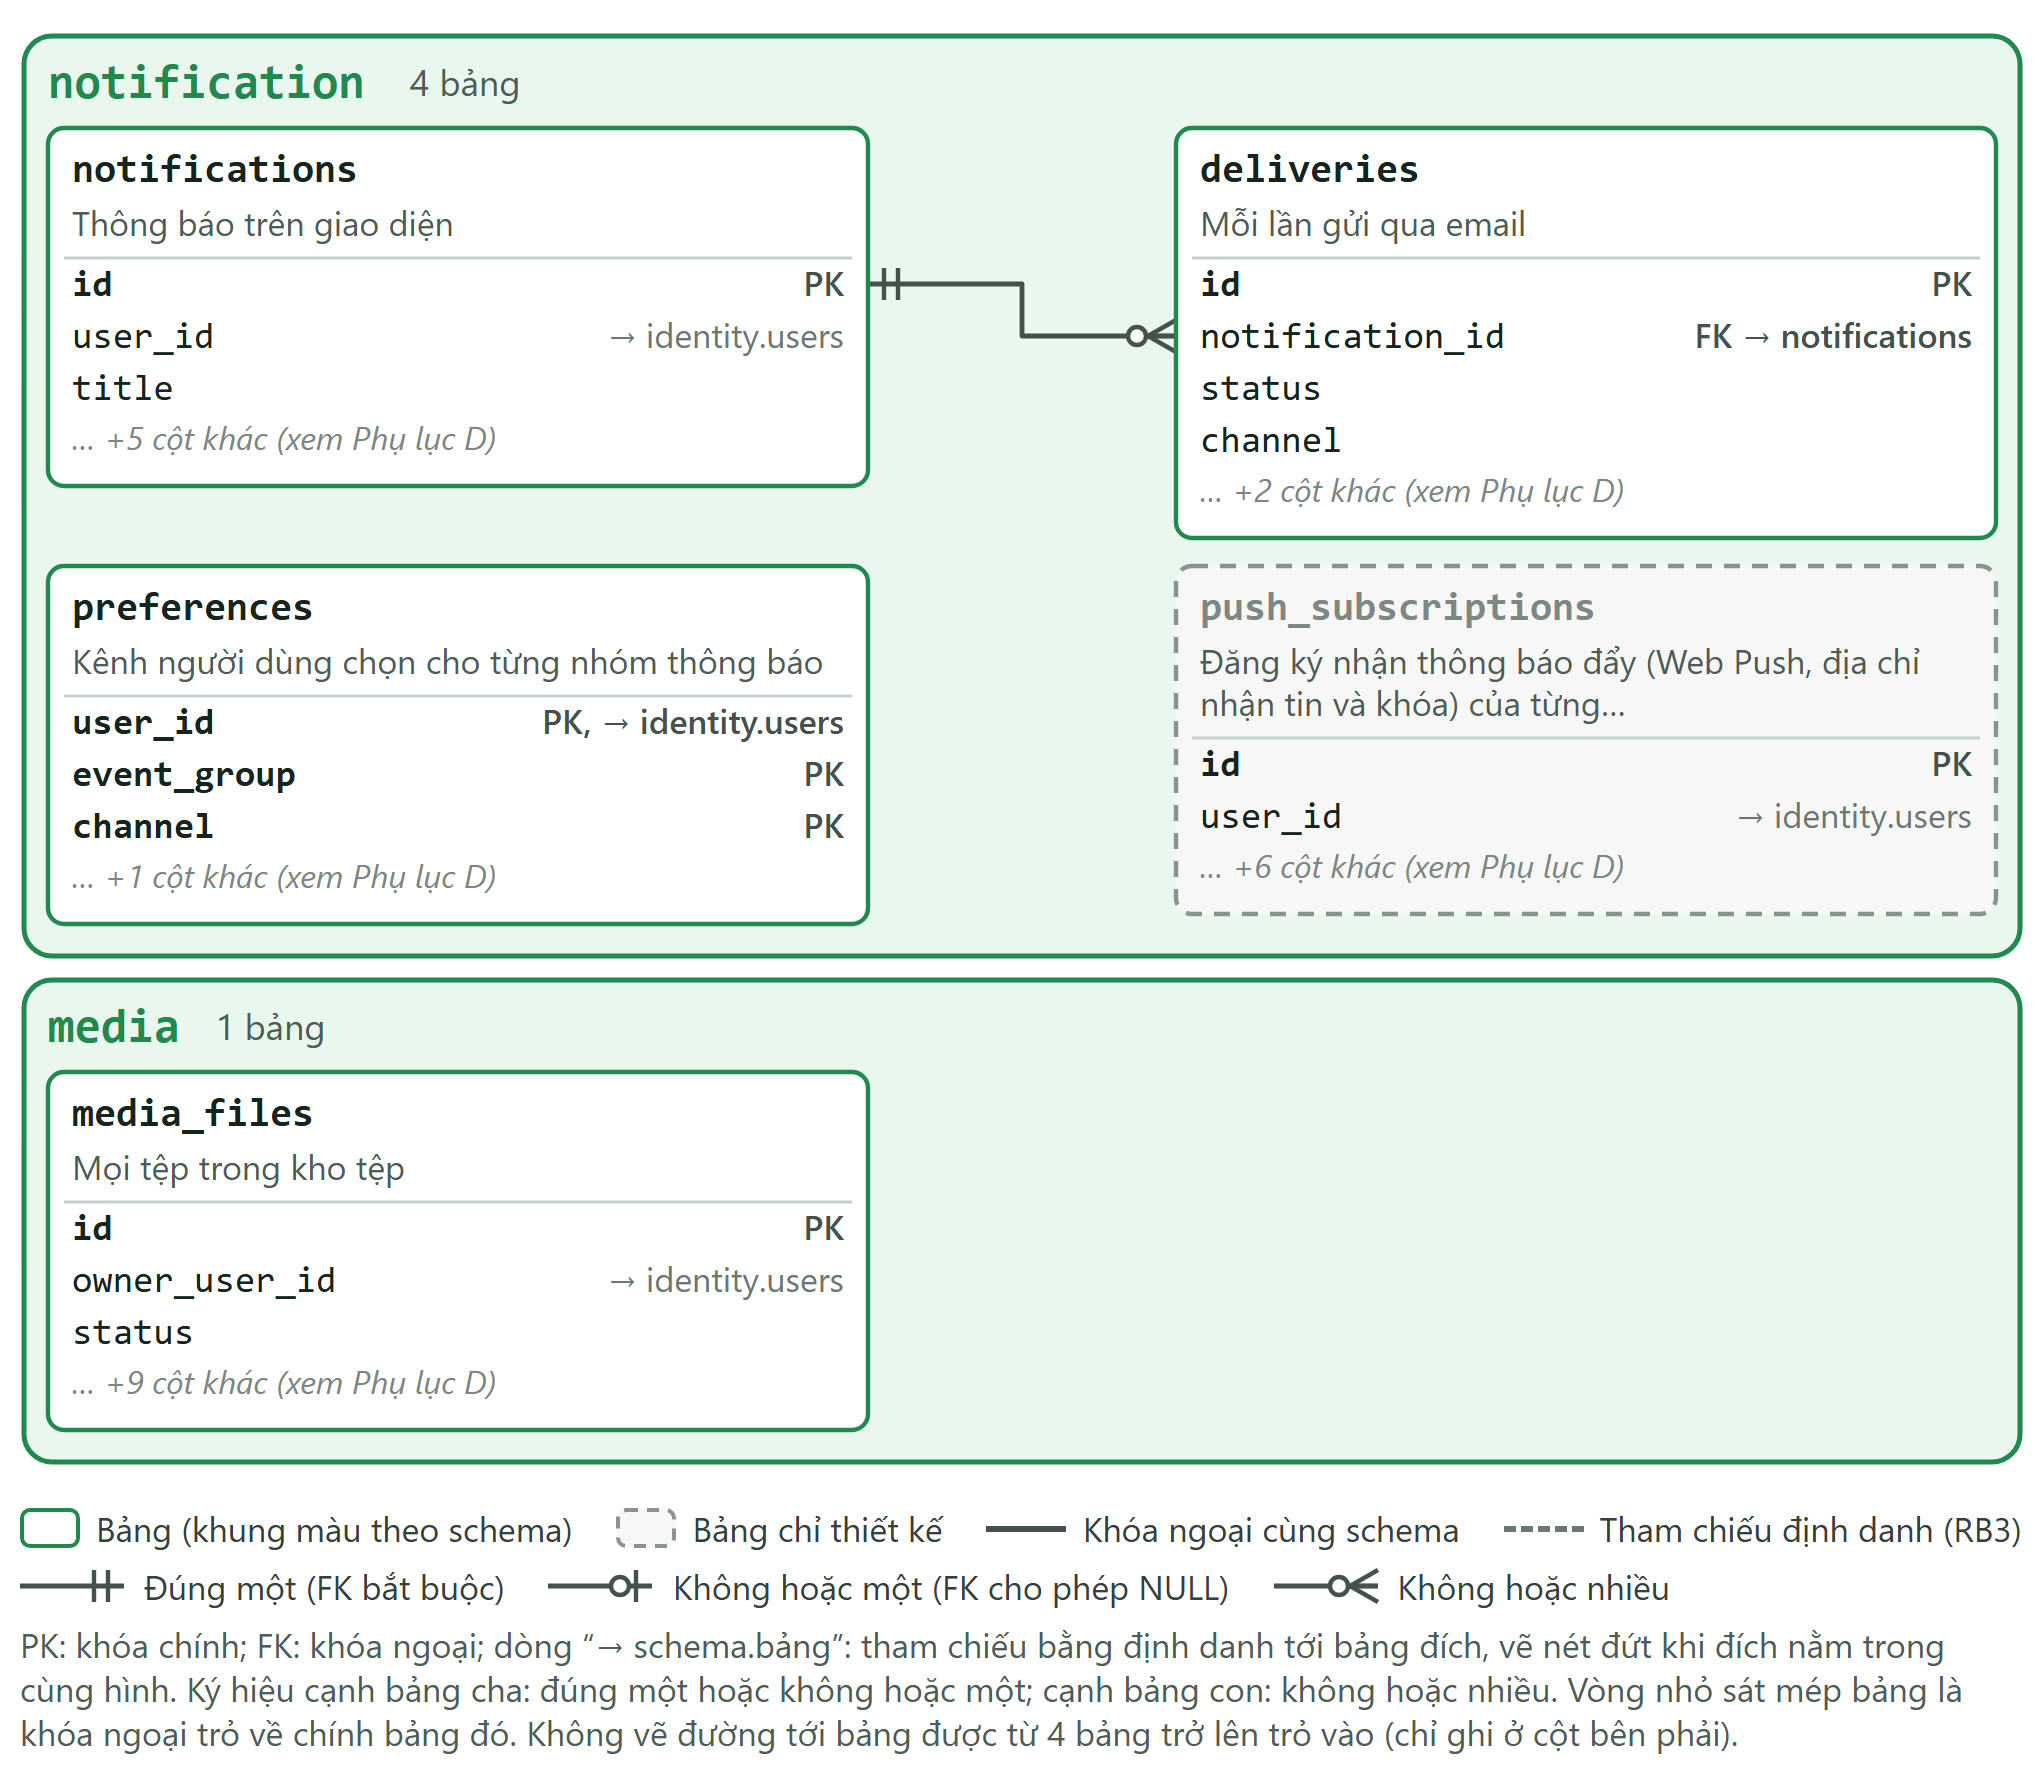
\includegraphics[width=\textwidth]{image/comparison/erd-thong-bao-tep.png}
\end{adjustbox}
\caption{ERD nền tảng chung, schema \texttt{notification} và \texttt{media} (5 bảng)}
\label{fig:erd-thong-bao-tep}
\end{figure}

\begin{figure}[t]
\centering
\begin{adjustbox}{max totalsize={\textwidth}{0.47\textheight},center}
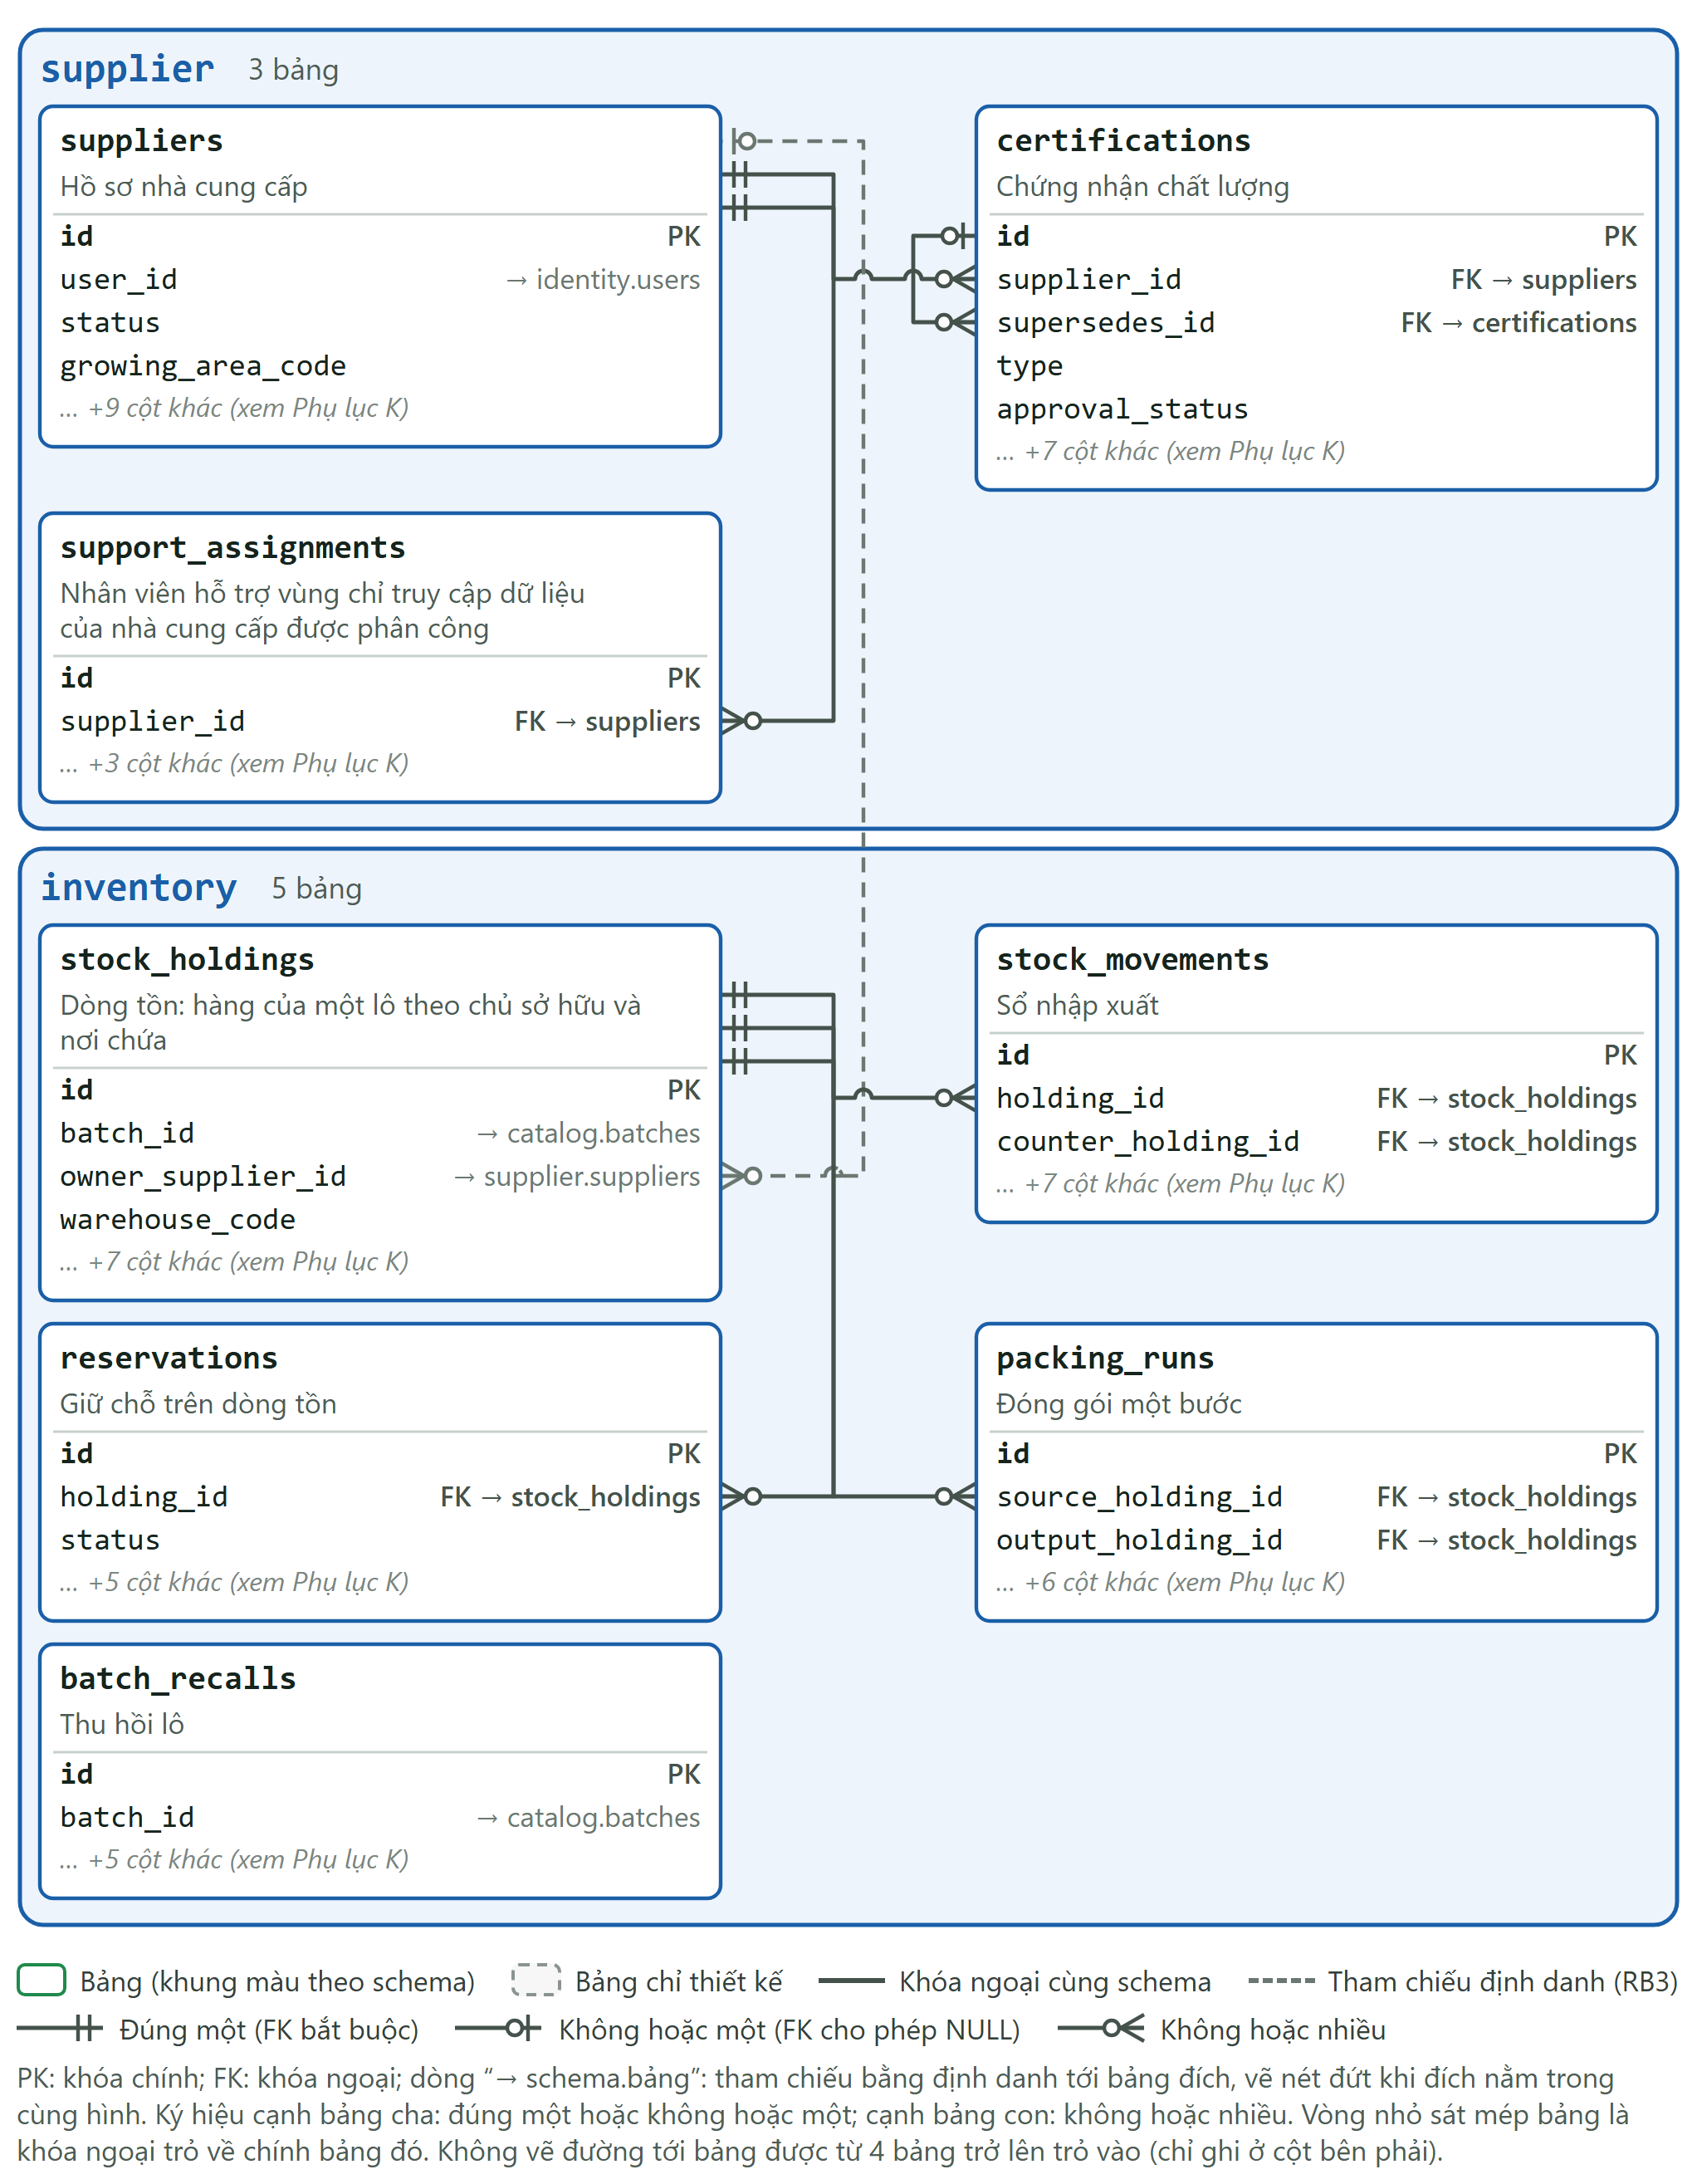
\includegraphics[width=\textwidth]{image/comparison/erd-nha-cung-cap-ton-kho.png}
\end{adjustbox}
\caption{ERD nguồn cung, schema \texttt{supplier} và \texttt{inventory} (8 bảng)}
\label{fig:erd-nha-cung-cap-ton-kho}
\end{figure}

\begin{figure}[t]
\centering
\begin{adjustbox}{max totalsize={\textwidth}{0.47\textheight},center}
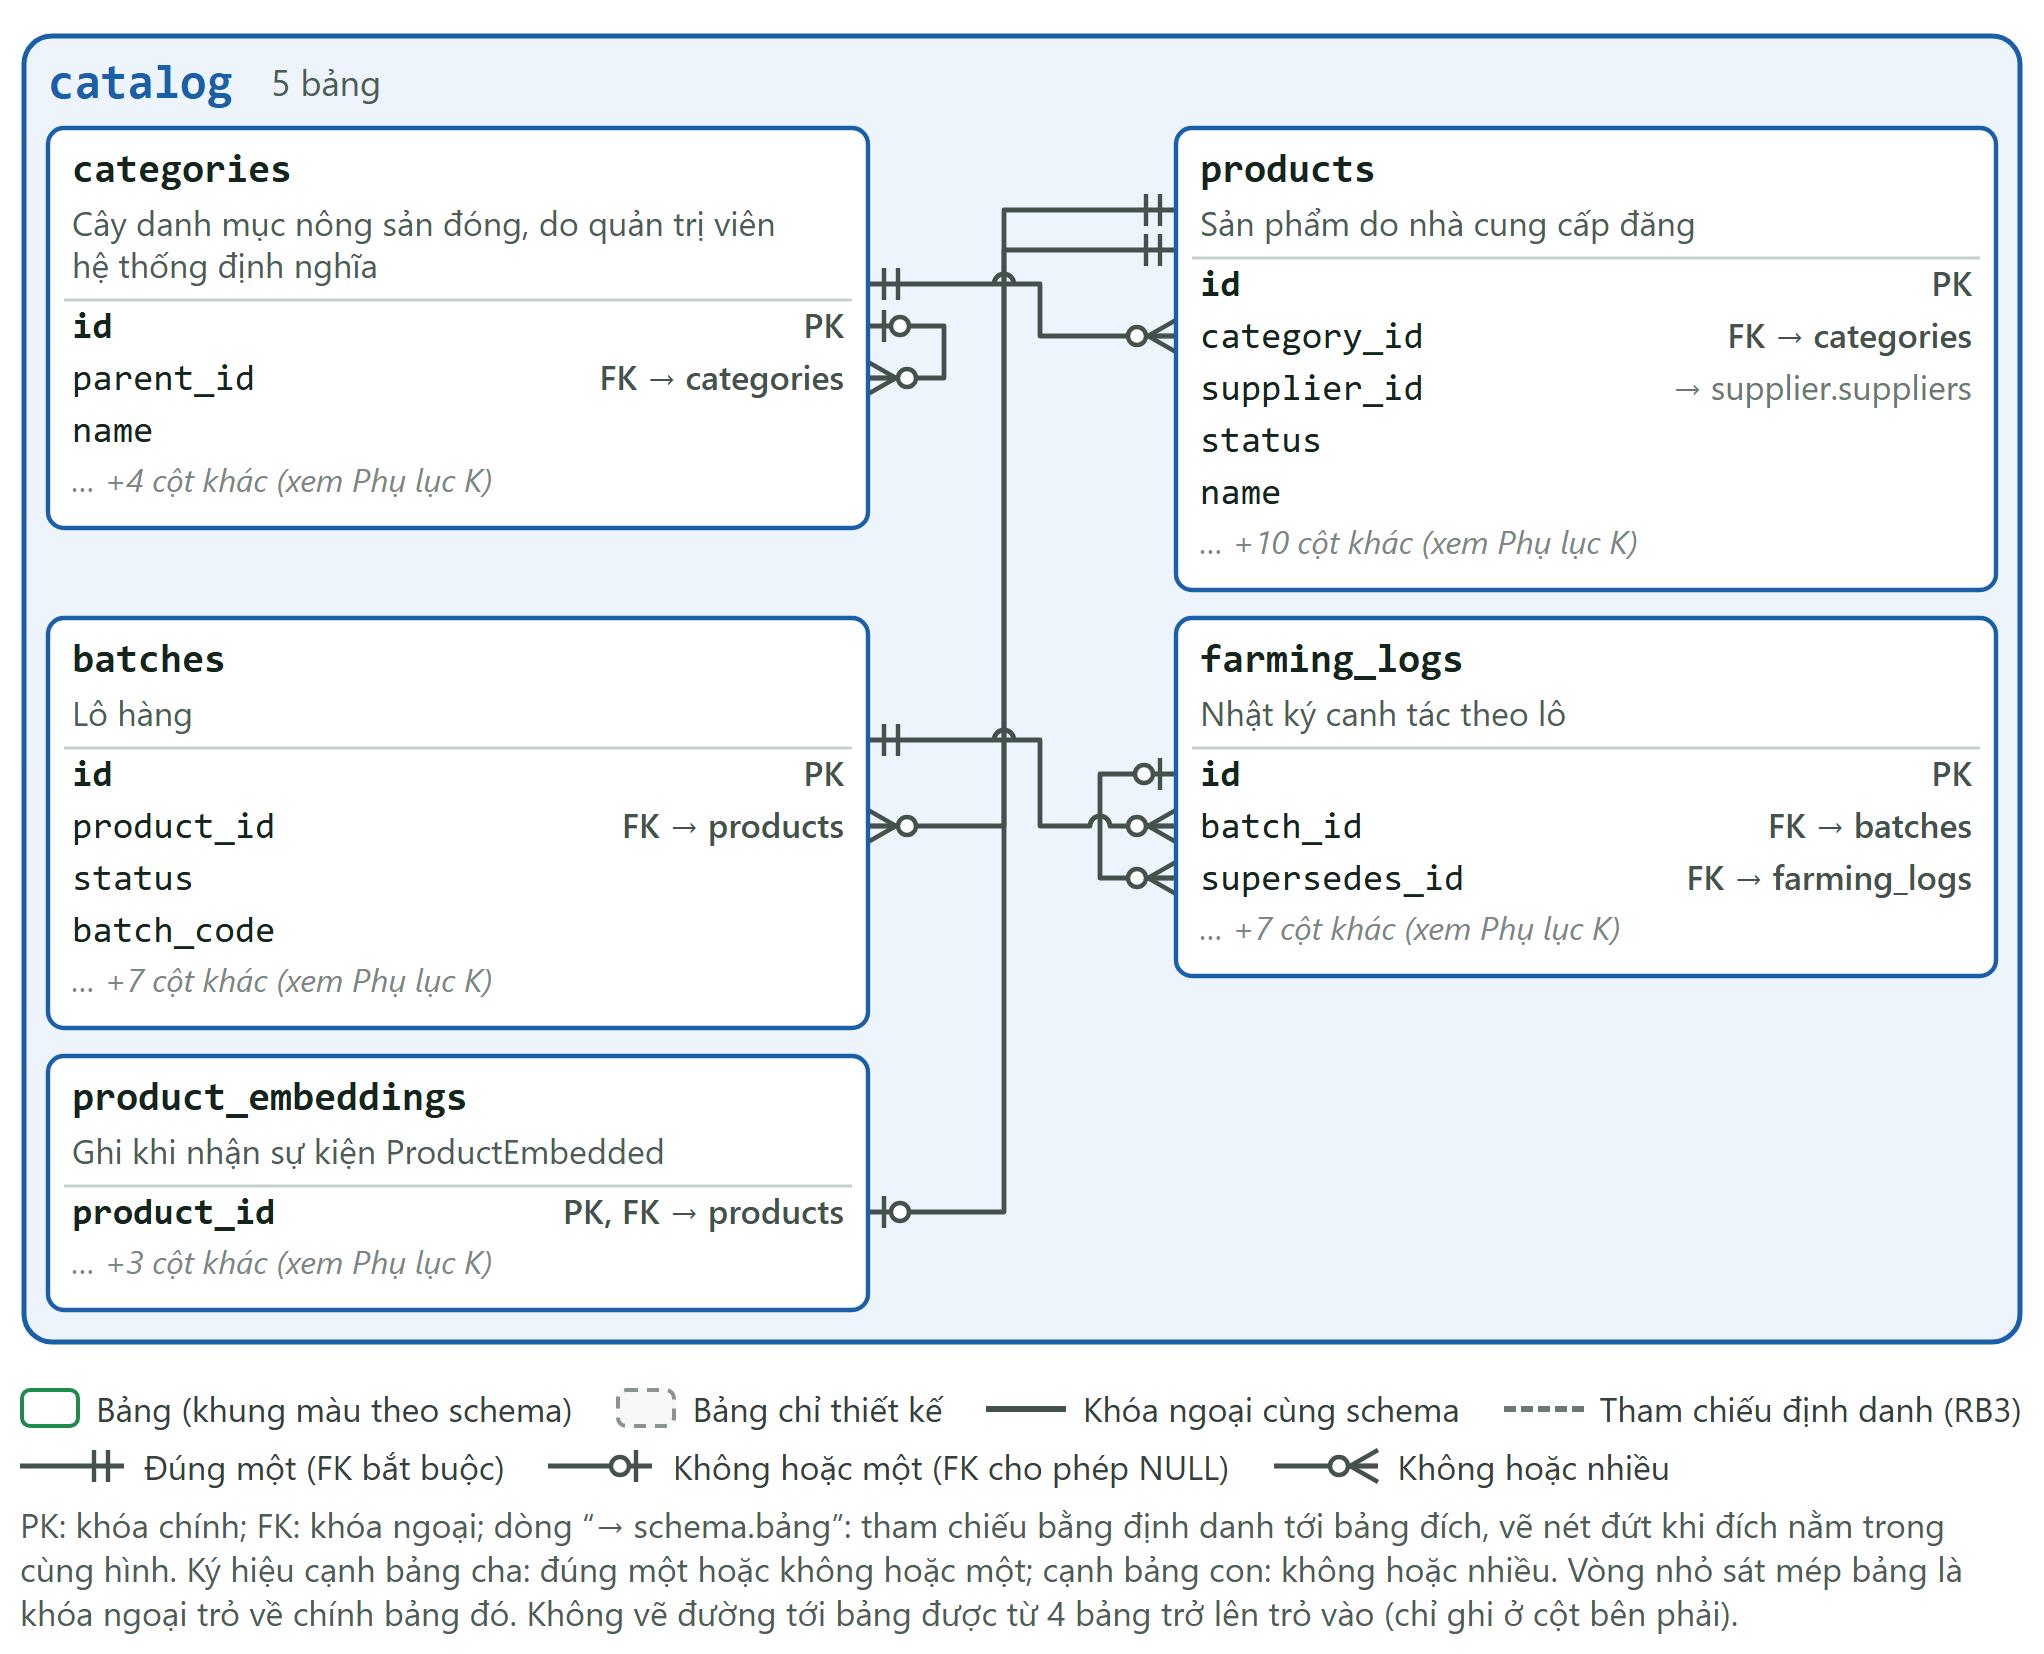
\includegraphics[width=\textwidth]{image/comparison/erd-danh-muc.png}
\end{adjustbox}
\caption{ERD nguồn cung, schema \texttt{catalog} (5 bảng)}
\label{fig:erd-danh-muc}
\end{figure}

\begin{figure}[t]
\centering
\begin{adjustbox}{max totalsize={\textwidth}{0.47\textheight},center}
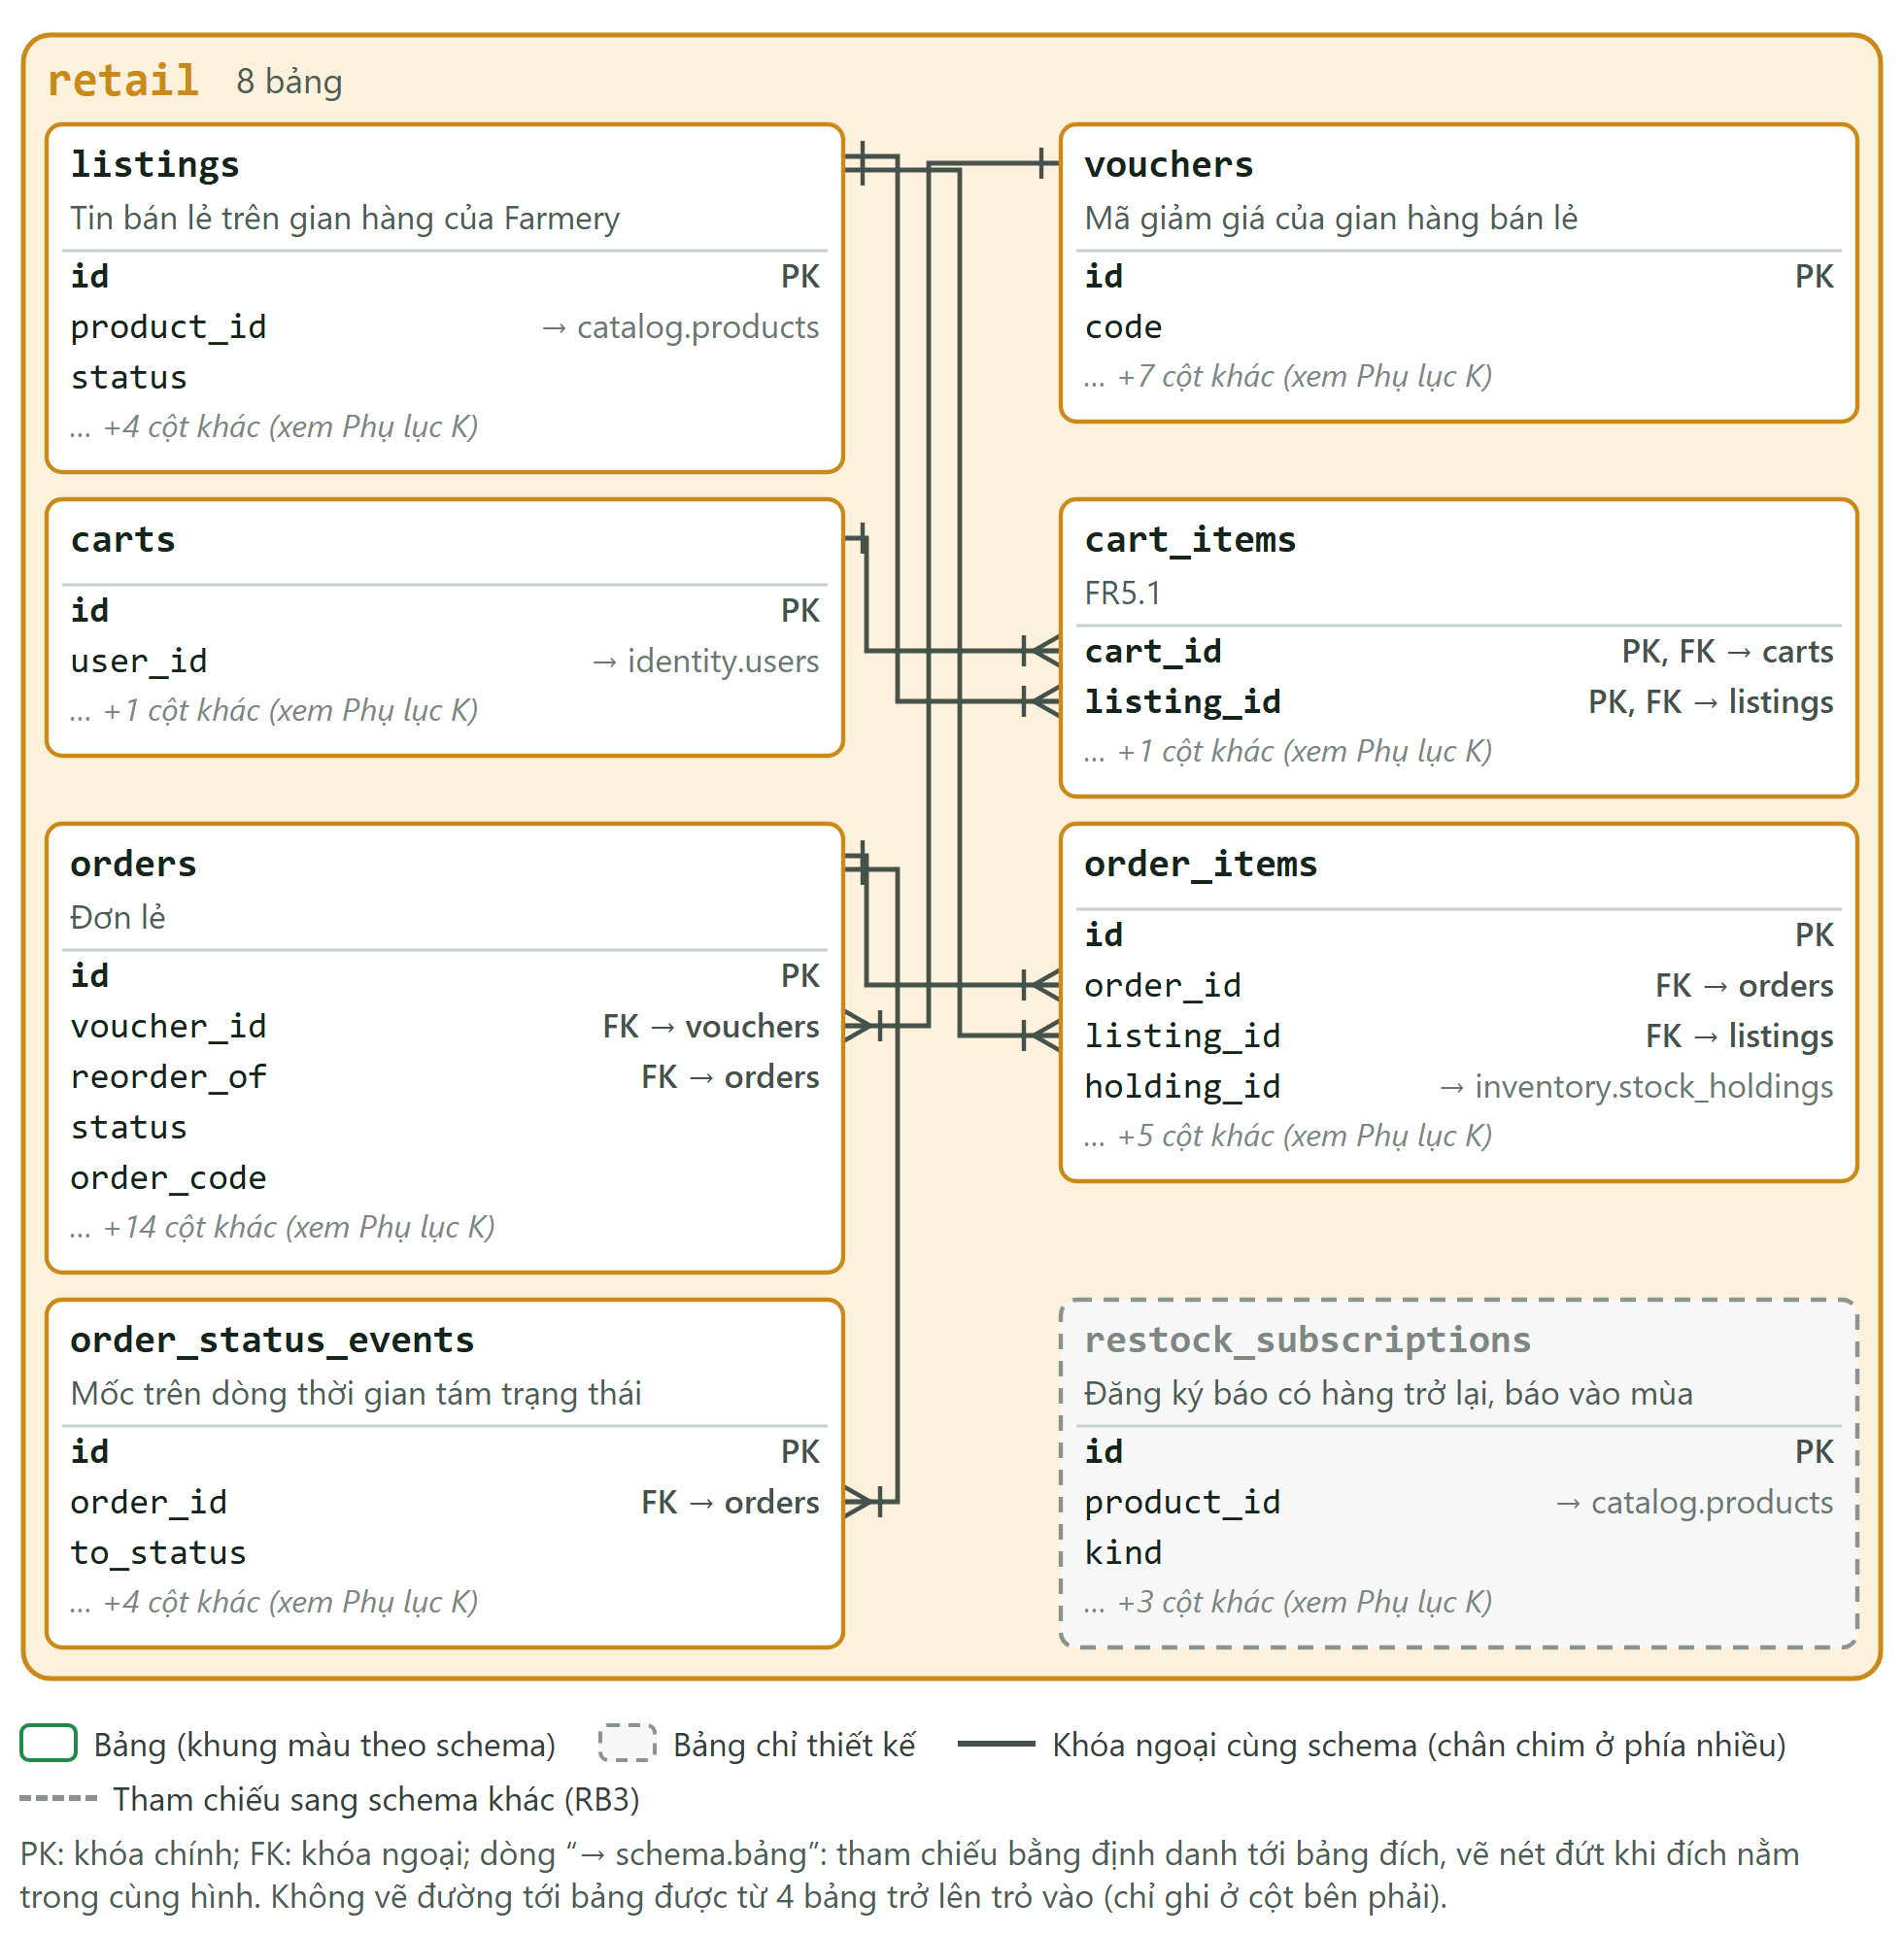
\includegraphics[width=\textwidth]{image/comparison/erd-ban-le.png}
\end{adjustbox}
\caption{ERD giao dịch, schema \texttt{retail} (8 bảng)}
\label{fig:erd-ban-le}
\end{figure}

\begin{figure}[t]
\centering
\begin{adjustbox}{max totalsize={\textwidth}{0.47\textheight},center}
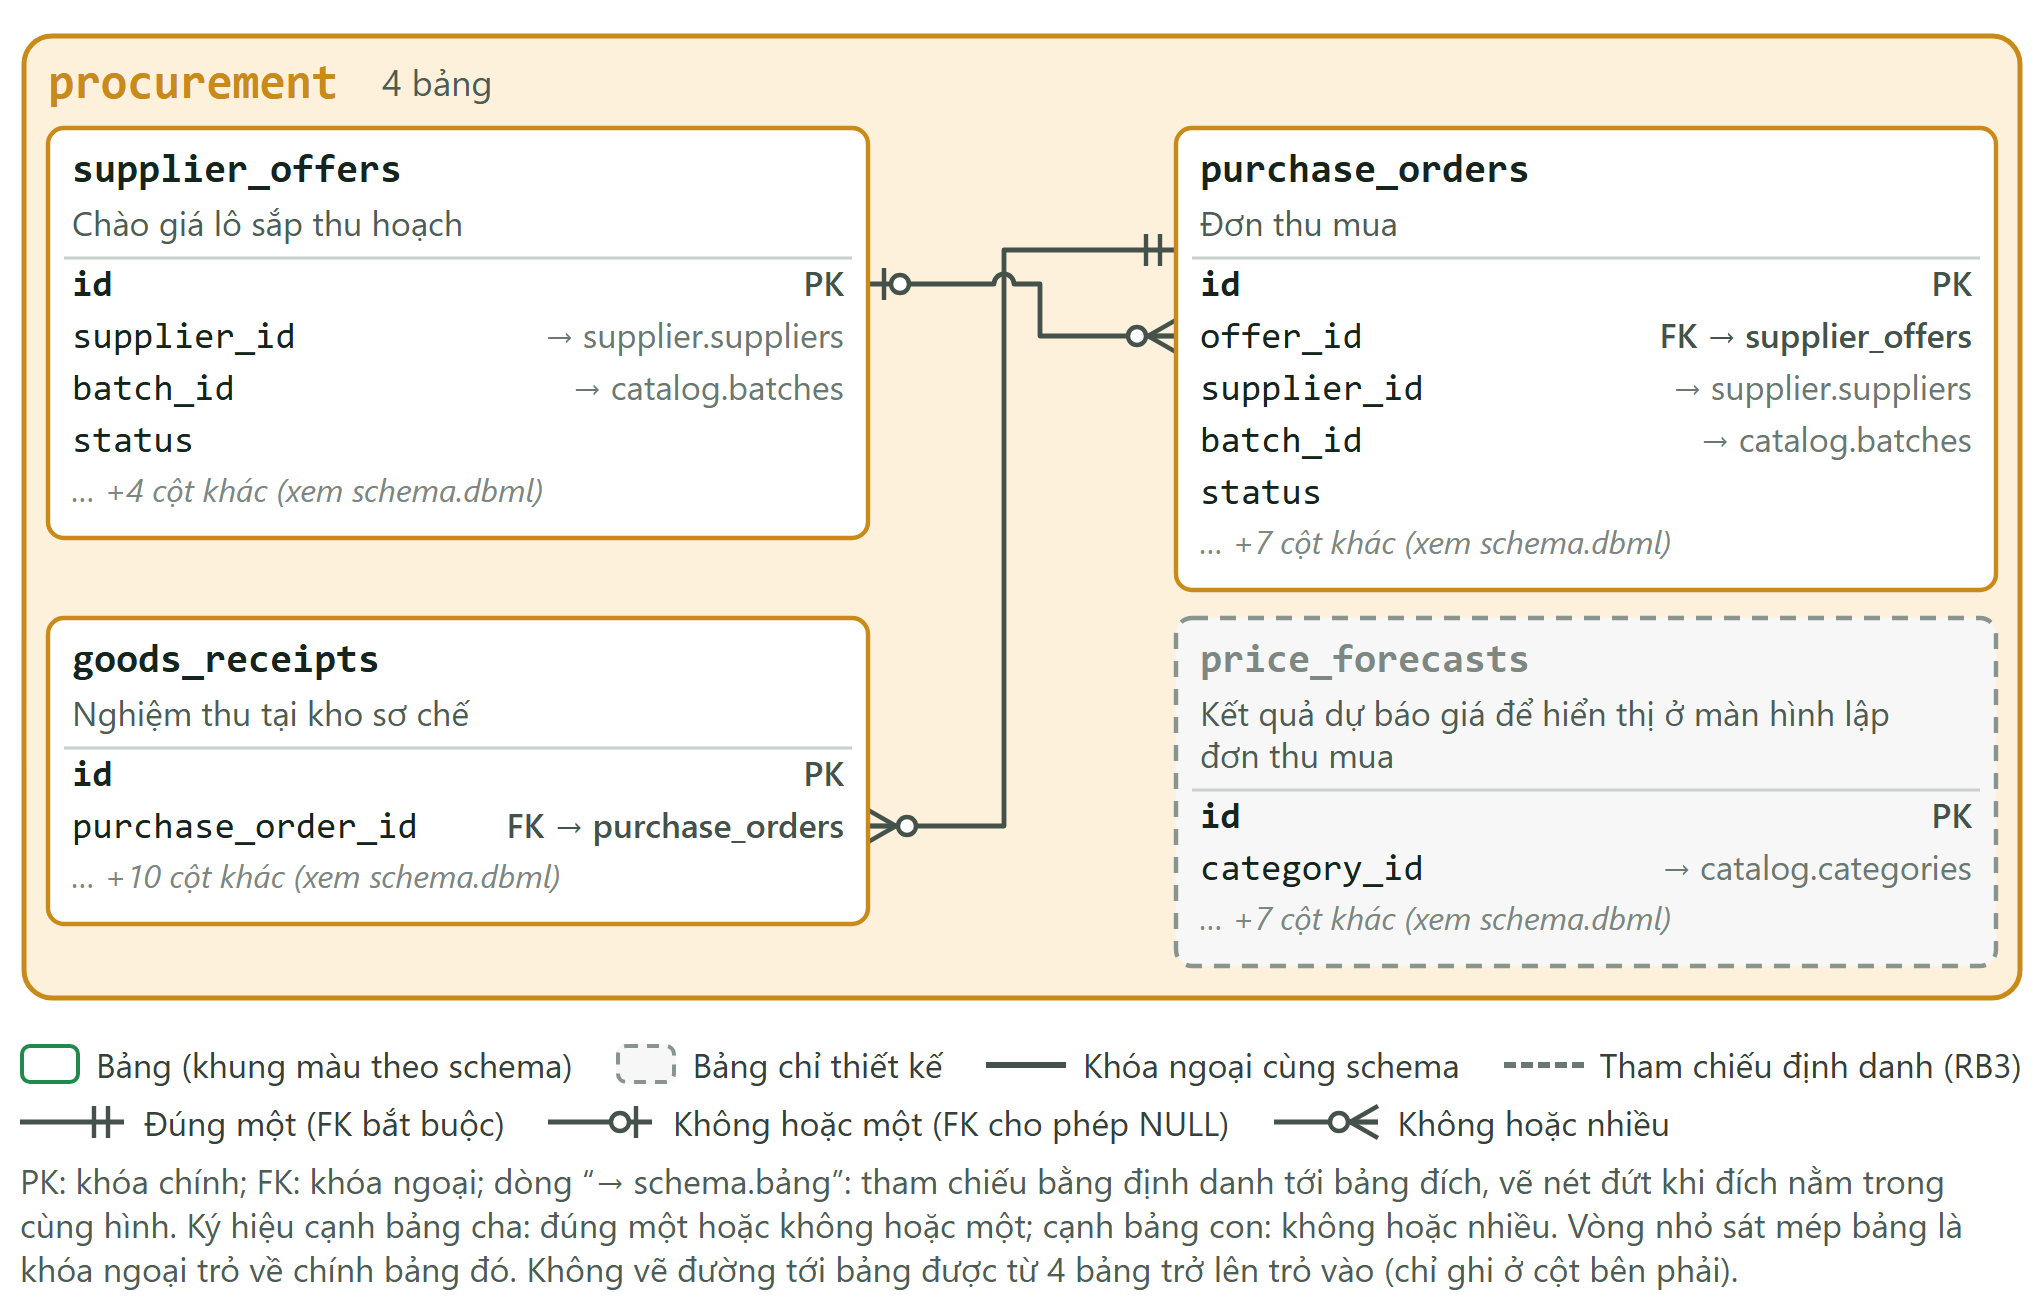
\includegraphics[width=\textwidth]{image/comparison/erd-thu-mua.png}
\end{adjustbox}
\caption{ERD giao dịch, schema \texttt{procurement} (4 bảng)}
\label{fig:erd-thu-mua}
\end{figure}

\begin{figure}[t]
\centering
\begin{adjustbox}{max totalsize={\textwidth}{0.47\textheight},center}
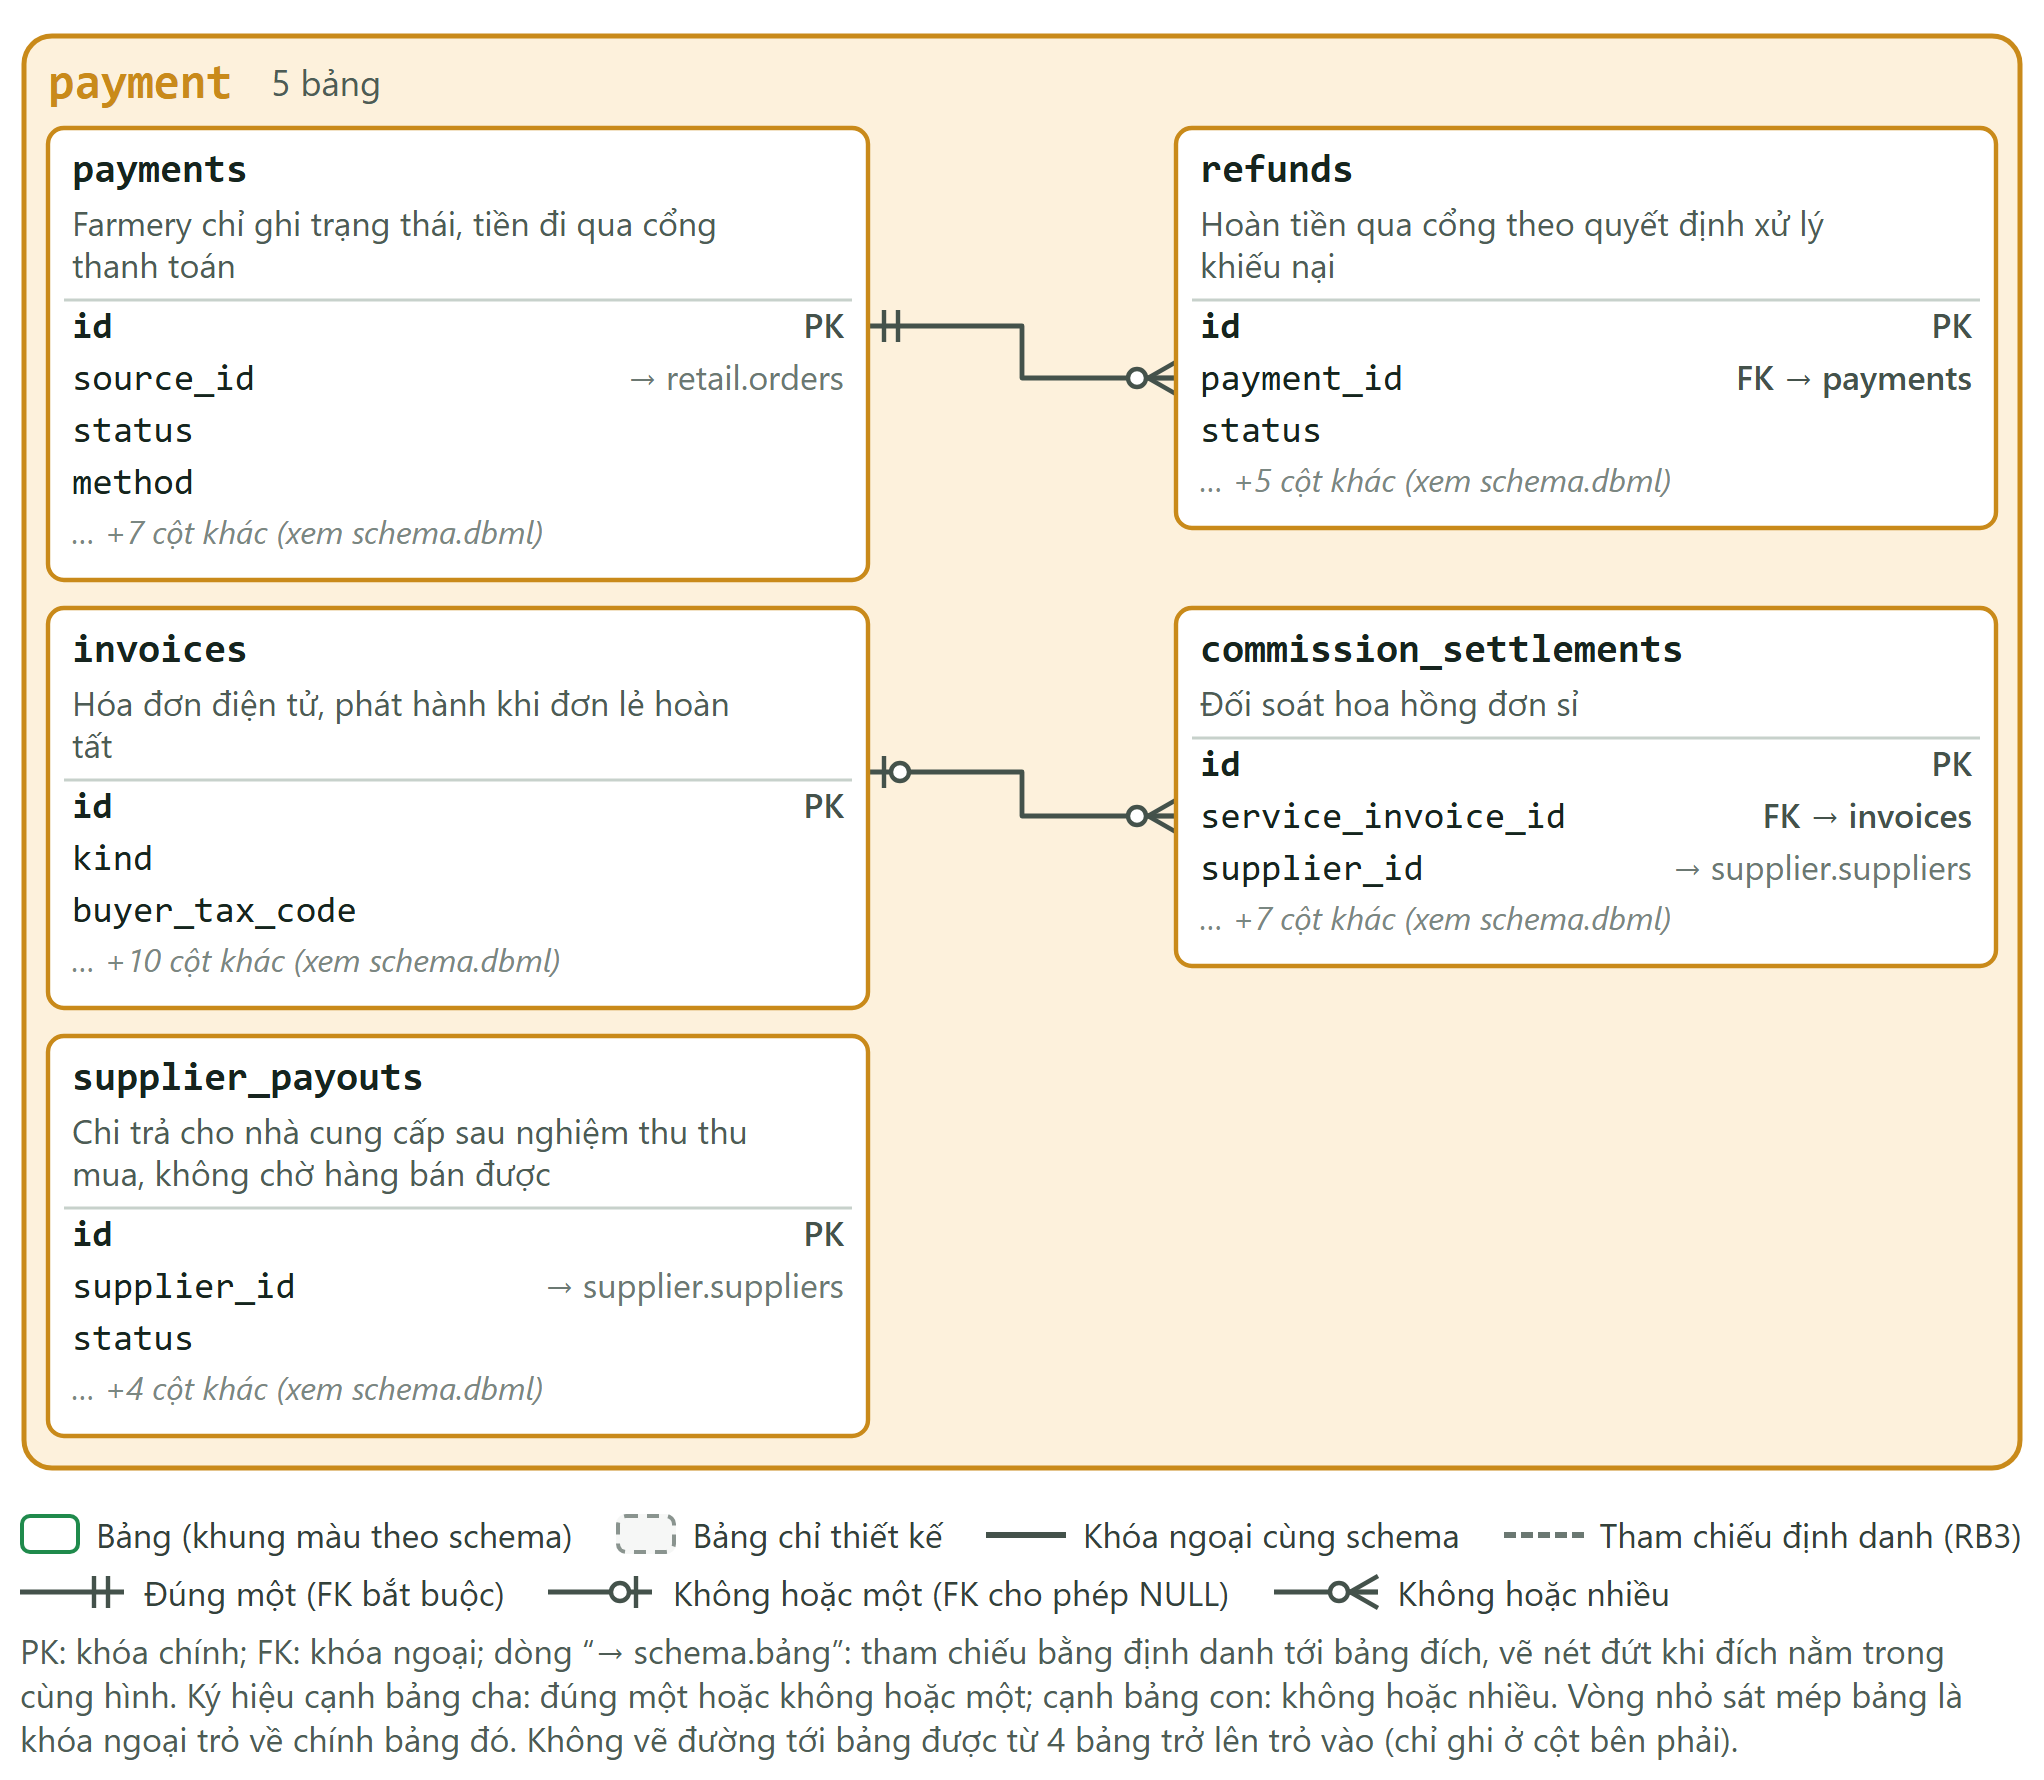
\includegraphics[width=\textwidth]{image/comparison/erd-thanh-toan.png}
\end{adjustbox}
\caption{ERD giao dịch, schema \texttt{payment} (5 bảng)}
\label{fig:erd-thanh-toan}
\end{figure}

\begin{figure}[t]
\centering
\begin{adjustbox}{max totalsize={\textwidth}{0.47\textheight},center}
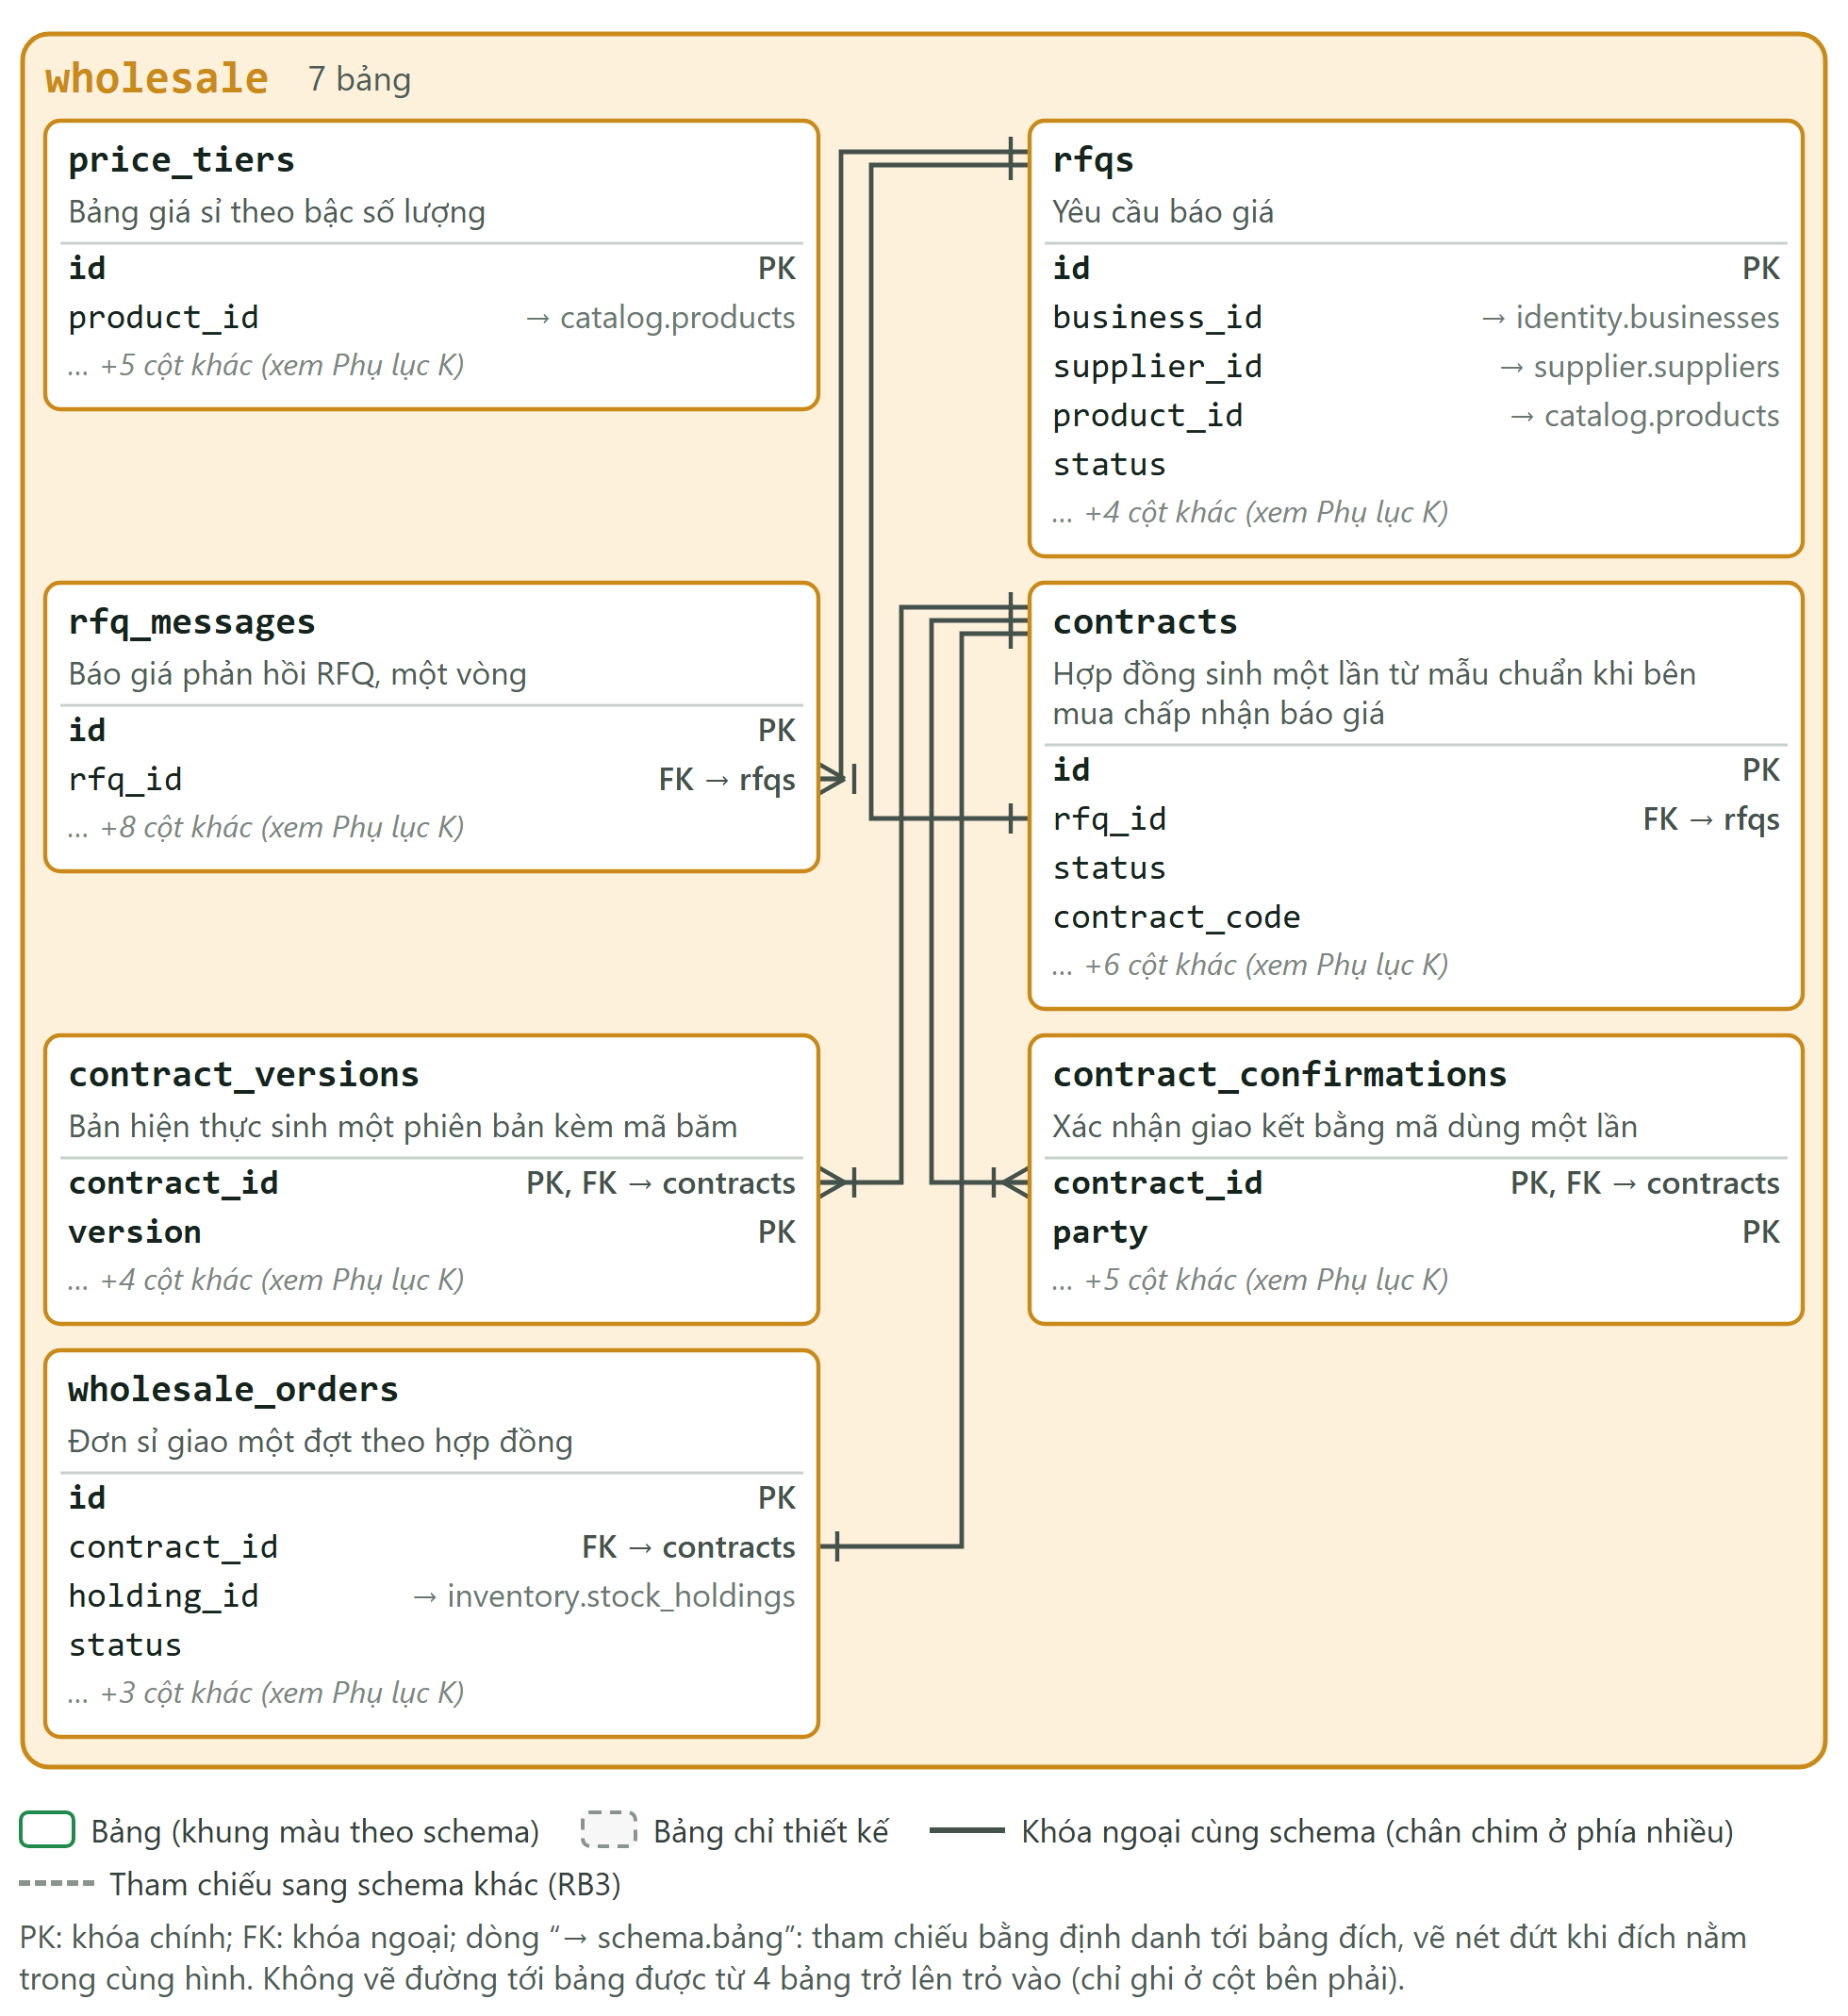
\includegraphics[width=\textwidth]{image/comparison/erd-ban-si.png}
\end{adjustbox}
\caption{ERD giao dịch, schema \texttt{wholesale} (7 bảng)}
\label{fig:erd-ban-si}
\end{figure}

\begin{figure}[t]
\centering
\begin{adjustbox}{max totalsize={\textwidth}{0.47\textheight},center}
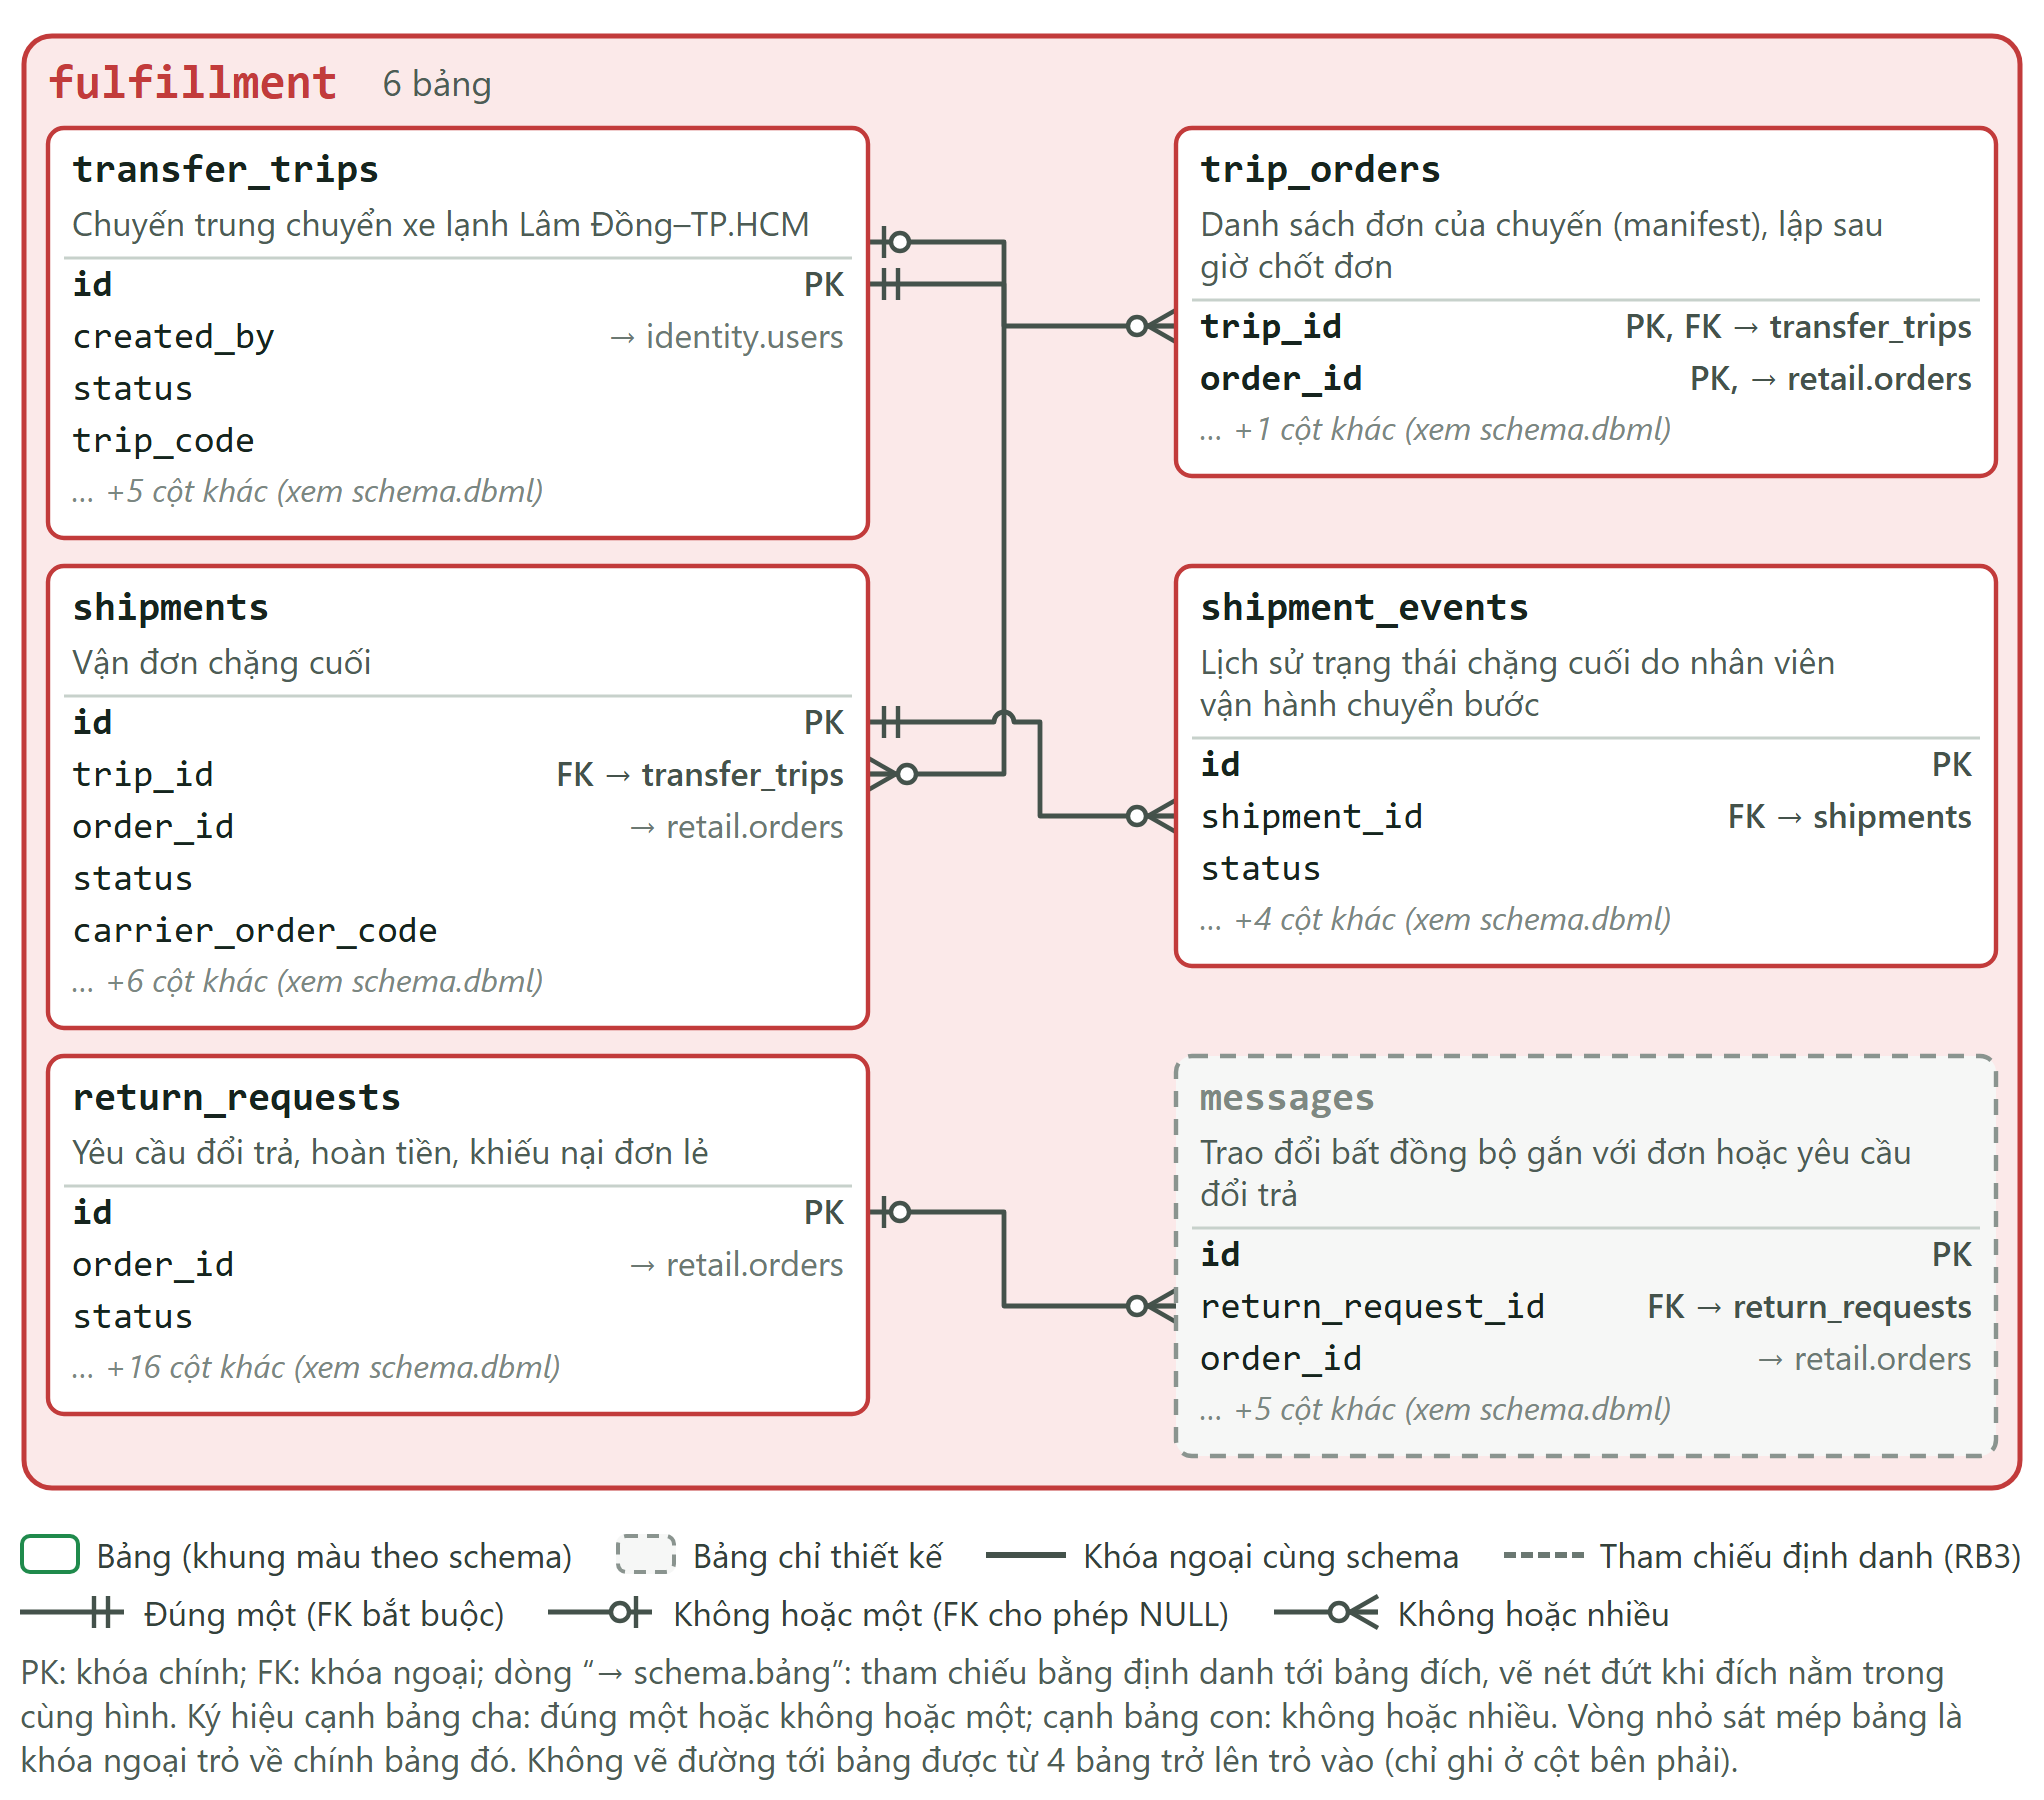
\includegraphics[width=\textwidth]{image/comparison/erd-giao-hang-doi-tra.png}
\end{adjustbox}
\caption{ERD sau bán, schema \texttt{fulfillment} (6 bảng)}
\label{fig:erd-giao-hang-doi-tra}
\end{figure}

\begin{figure}[t]
\centering
\begin{adjustbox}{max totalsize={\textwidth}{0.47\textheight},center}
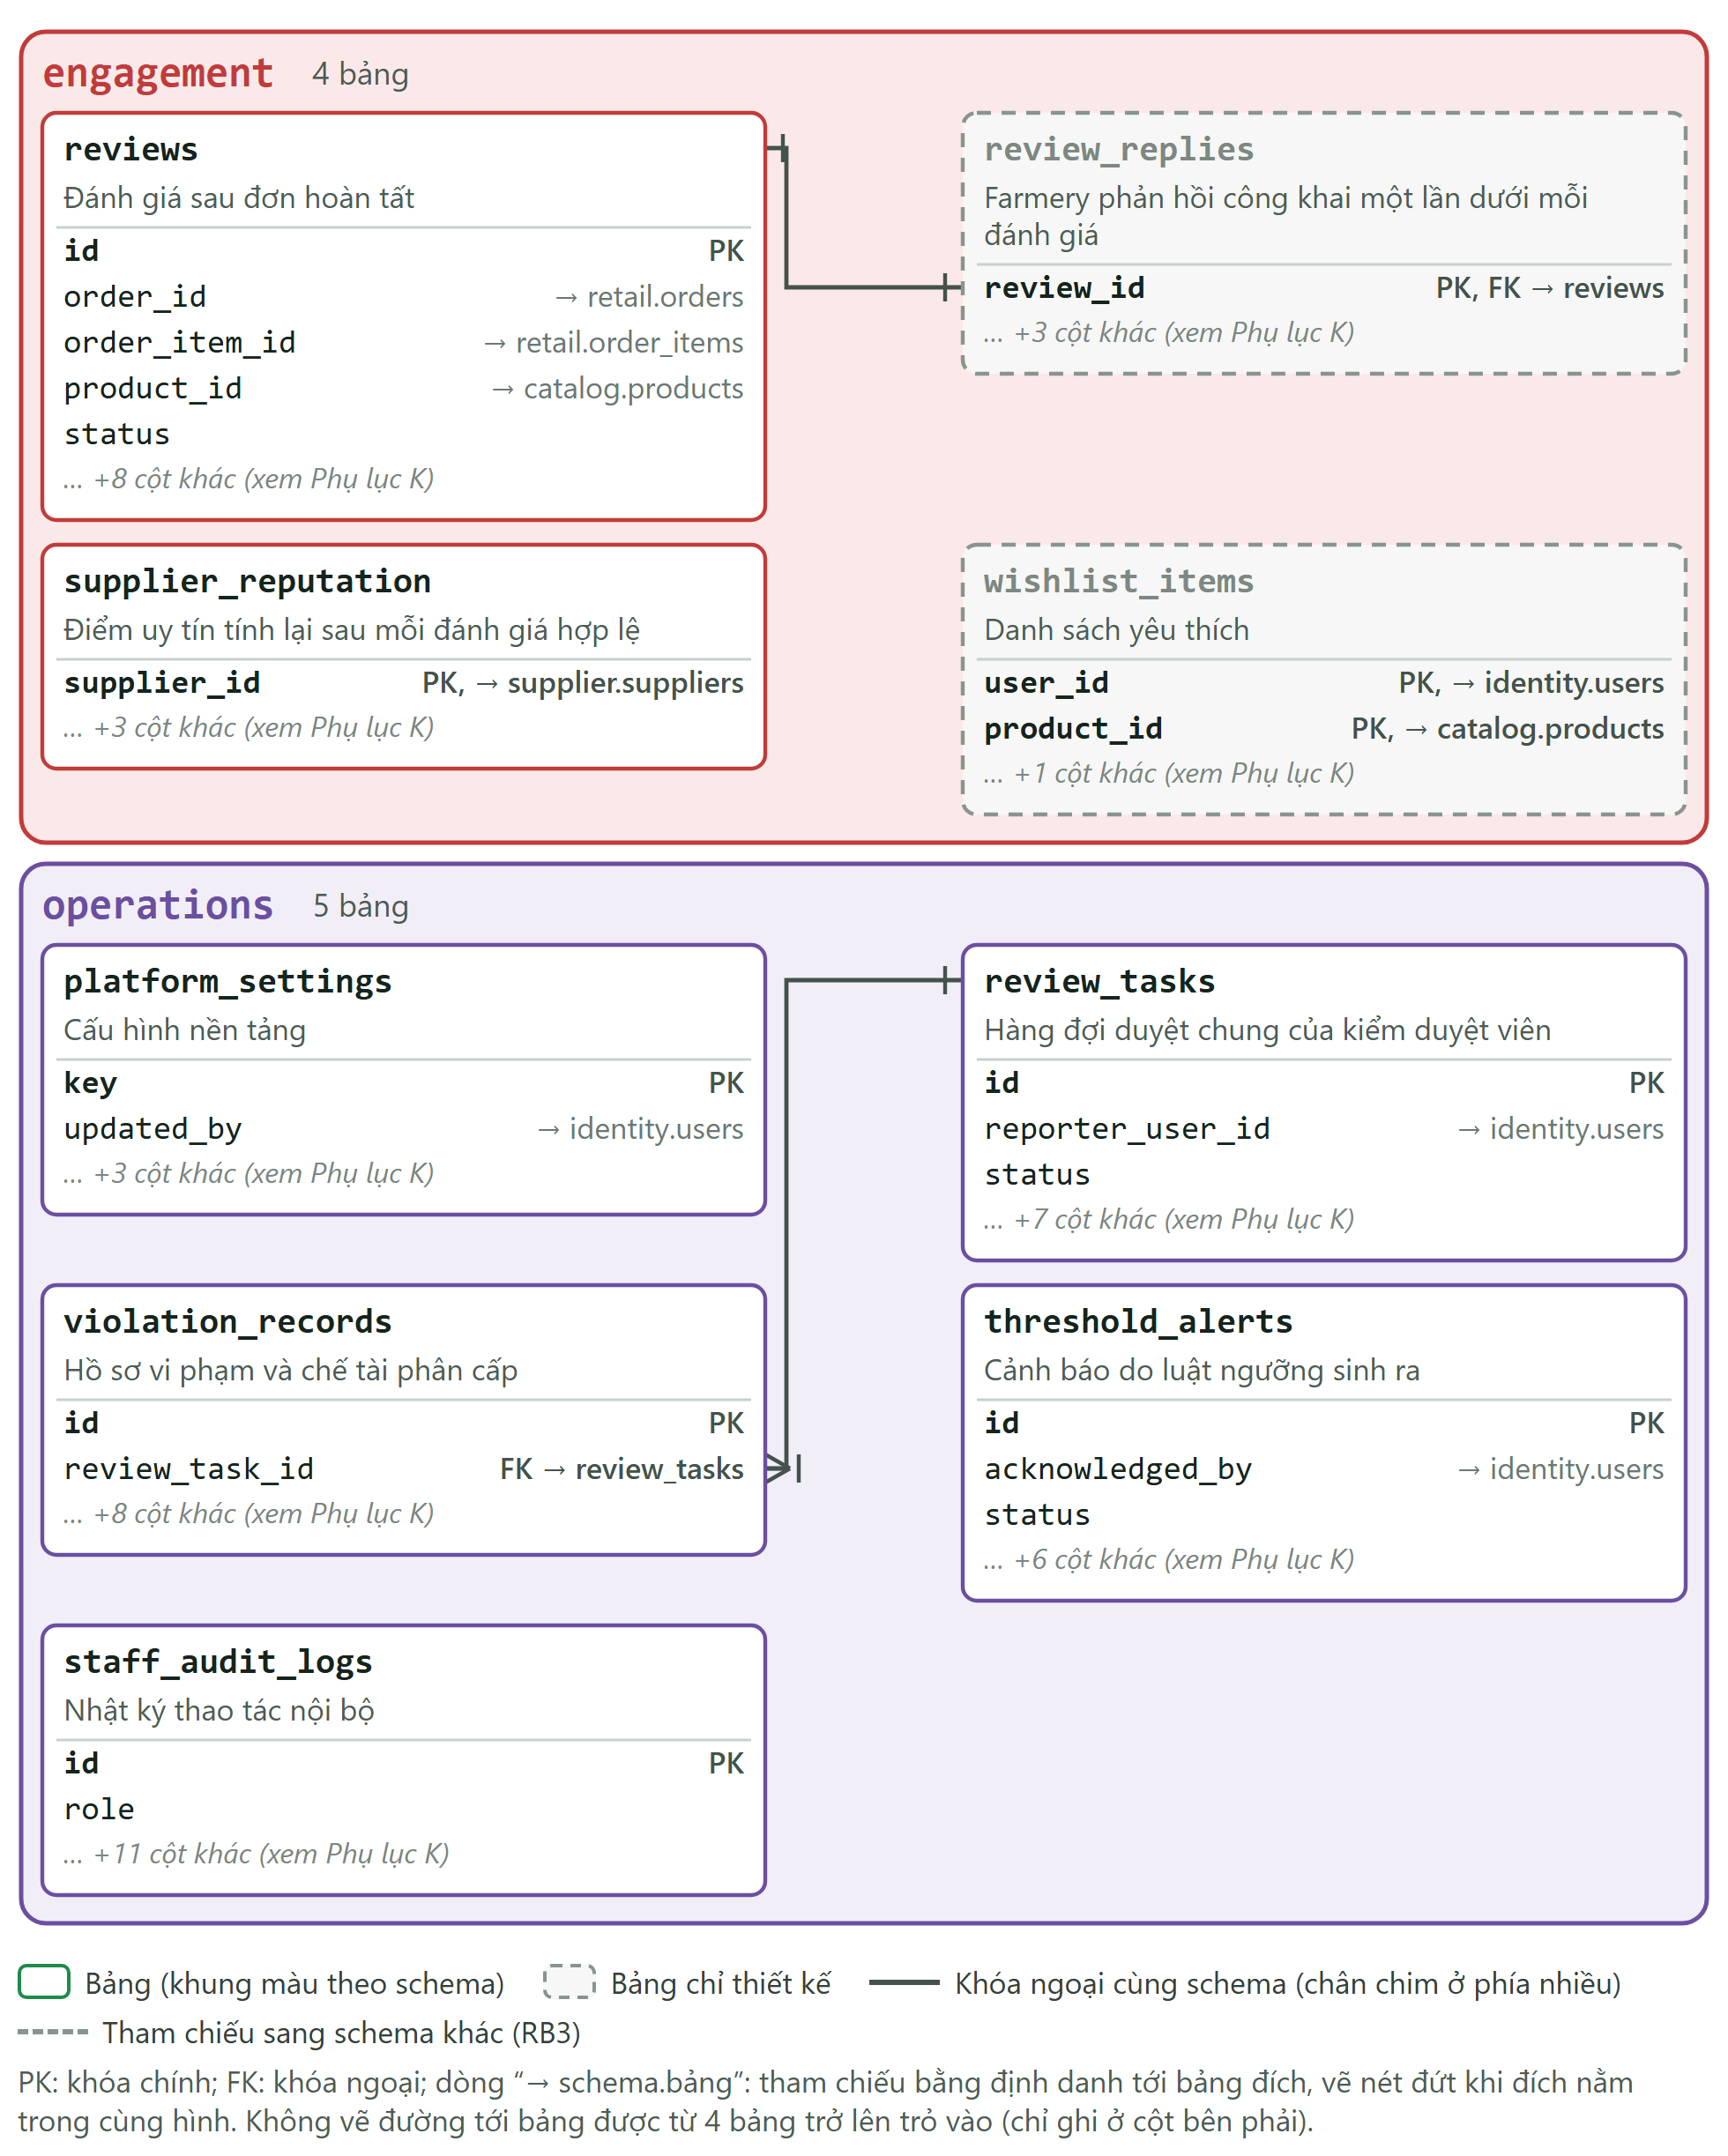
\includegraphics[width=\textwidth]{image/comparison/erd-danh-gia-van-hanh.png}
\end{adjustbox}
\caption{ERD sau bán, schema \texttt{engagement} (4 bảng), và vận hành, schema \texttt{operations} (5 bảng)}
\label{fig:erd-danh-gia-van-hanh}
\end{figure}
